%%%%%%%%%%%%%%%%%%%%%%%%%%%%%%%%%%%%%%%%%
% Short Sectioned Assignment
% LaTeX Template
% Version 1.0 (5/5/12)
%
% This template has been downloaded from:
% http://www.LaTeXTemplates.com
%
% Original author:
% Frits Wenneker (http://www.howtotex.com)
%
% License:
% CC BY-NC-SA 3.0 (http://creativecommons.org/licenses/by-nc-sa/3.0/)
%
%%%%%%%%%%%%%%%%%%%%%%%%%%%%%%%%%%%%%%%%%

%----------------------------------------------------------------------------------------
%	PACKAGES AND OTHER DOCUMENT CONFIGURATIONS
%----------------------------------------------------------------------------------------

\documentclass[paper=a4, fontsize=11pt]{scrartcl} % A4 paper and 11pt font size

\usepackage{fourier} % Use the Adobe Utopia font for the document - comment this line to return to the LaTeX default
\usepackage[french]{babel} % English language/hyphenation
\usepackage{amsmath,amsfonts,amsthm} % Math packages

\usepackage{lipsum} % Used for inserting dummy 'Lorem ipsum' text into the template
\usepackage{graphicx}
\usepackage{sectsty} % Allows customizing section commands
\allsectionsfont{\centering \normalfont\scshape} % Make all sections centered, the default font and small caps

% tentative pour les algorithmes 
\usepackage{algorithm}
\usepackage{algpseudocode}

\usepackage{fancyhdr} % Custom headers and footers
\pagestyle{fancyplain} % Makes all pages in the document conform to the custom headers and footers
\fancyhead{} % No page header - if you want one, create it in the same way as the footers below
\fancyfoot[L]{} % Empty left footer
\fancyfoot[C]{} % Empty center footer
\fancyfoot[R]{\thepage} % Page numbering for right footer
\renewcommand{\headrulewidth}{0pt} % Remove header underlines
\renewcommand{\footrulewidth}{0pt} % Remove footer underlines
\setlength{\headheight}{13.6pt} % Customize the height of the header

\numberwithin{equation}{section} % Number equations within sections (i.e. 1.1, 1.2, 2.1, 2.2 instead of 1, 2, 3, 4)
\numberwithin{figure}{section} % Number figures within sections (i.e. 1.1, 1.2, 2.1, 2.2 instead of 1, 2, 3, 4)
\numberwithin{table}{section} % Number tables within sections (i.e. 1.1, 1.2, 2.1, 2.2 instead of 1, 2, 3, 4)

\setlength\parindent{0pt} % Removes all indentation from paragraphs - comment this line for an assignment with lots of text

%----------------------------------------------------------------------------------------
%	TITLE SECTION
%----------------------------------------------------------------------------------------

\newcommand{\horrule}[1]{\rule{\linewidth}{#1}} % Create horizontal rule command with 1 argument of height

\title{	
\normalfont \normalsize 
\textsc{Ecole Centrale de Nantes} \\ [25pt] % Your university, school and/or department name(s)
\horrule{0.5pt} \\[0.4cm] % Thin top horizontal rule
\huge Option Informatique - Corrigé TD MADIS \\ % The assignment title
\horrule{2pt} \\[0.5cm] % Thick bottom horizontal rule
}

%\author{Durée 1h - Aucun document autorisé} % Your name

%\date{\normalsize\today} % Today's date or a custom date

\begin{document}

\maketitle % Print the title

\section{L'itinéraire de Michel Strogoff}

\subsection{Itinéraire}

Dans cette première partie, on va appliquer une version légèrement modifiée de l'algorithme de Ford-Bellman. C'est possible car notre graphe ne comporte pas de boucles, cf figure~\ref{fig:ms}.

\begin{figure}[htbp]
\begin{center}
	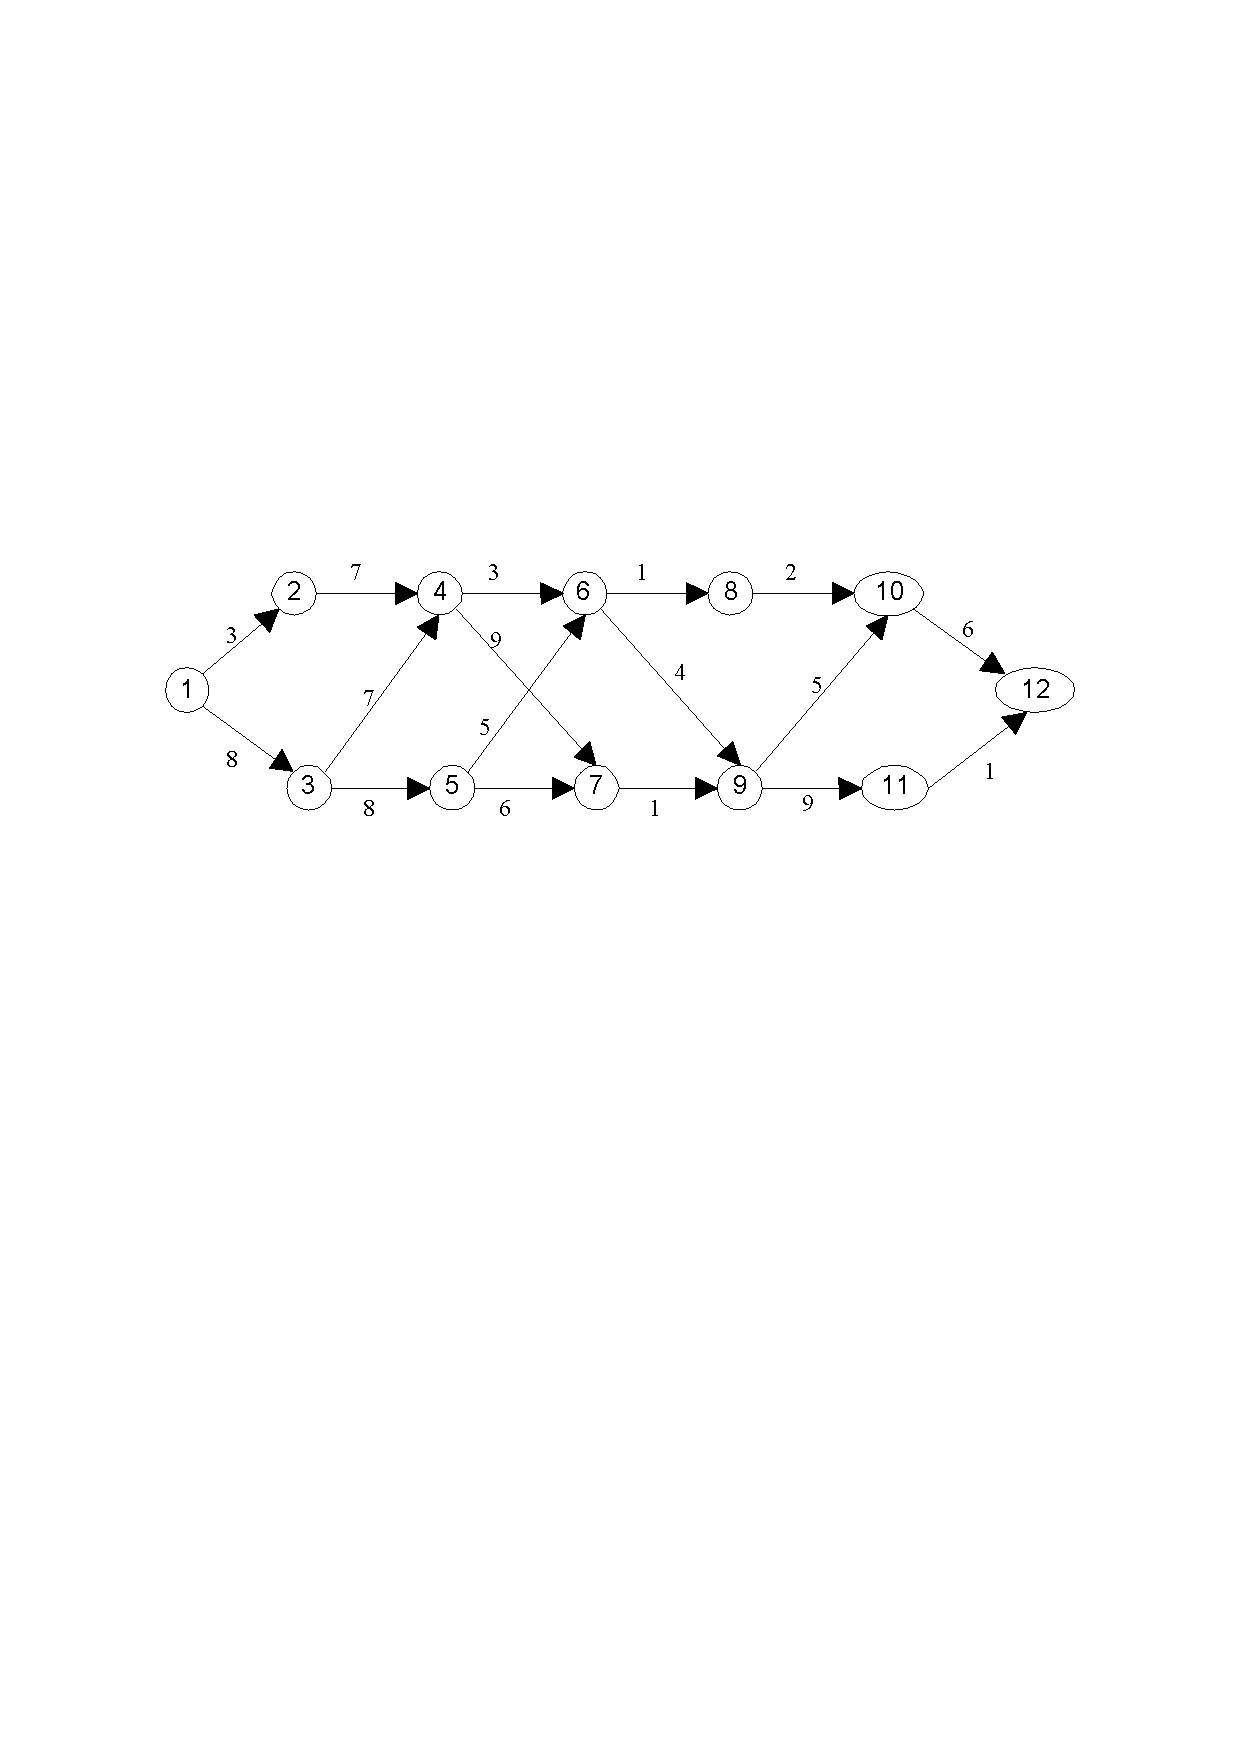
\includegraphics[width=.8\textwidth]{strogoff.pdf}
	\caption{Itinéraires possibles et chances de succès pour un trajet d'une ville à l'autre}
	\label{fig:ms}
\end{center}
\end{figure}

La seule modification à apporter à l'algorithme ordinal consiste à remplacer le min par un max. 


\begin{table}[htbp]
  \begin{center}
    \begin{tabular}{cccccccccccc}
      \hline
      $\epsilon$ & 1 & 1 & 3 & 3 & 5 & 4 & 6 & 6,7 & 9 & 9 & 10 \\
      \hline
      1 & 2 & 3 & 4 & 5 & 6 & 7 & 8 & 9 & 10 & 11 & 12 \\
      \hline
      0  \\
      0 & 3  \\
      0 & 3 & 8 \\
      0 & 3 & 8 & 15 \\
      0 & 3 & 8 & 15 & 16\\
      0 & 3 & 8 & 15 & 16 & 21 \\
      0 & 3 & 8 & 15 & 16 & 21 & 24\\
      0 & 3 & 8 & 15 & 16 & 21 & 24 & 22 \\
      0 & 3 & 8 & 15 & 16 & 21 & 24 & 22 & 25 \\
      0 & 3 & 8 & 15 & 16 & 21 & 24 & 22 & 25 & 30 \\
      0 & 3 & 8 & 15 & 16 & 21 & 24 & 22 & 25 & 30 & 34 \\
      0 & 3 & 8 & 15 & 16 & 21 & 24 & 24 & 25 & 30 & 34 & 36 \\
    \end{tabular}
  \end{center}
  \caption{Tableau des itérations de l'algorithme}
  \label{tab:fb}
\end{table}

Si on remonte à partir du sommet 12, on obtient deux chemins de longueur équivalente :
\begin{itemize}
\item 12-10-9-6-5-3-1
\item 12-10-9-7-4-3-1
\end{itemize}

\subsection{Probabilité de succès}

Ici, on se contente de considérer que $x$ chances sur $10$ de succès constituent une probabilité de $\frac{x}{10}$ de succès et que toutes les variables sont indépendantes. 

Dans le premier cas, nous obtenons alors une probabilité $p_1=0.0384$, tandis que pour le second, nous avons $p_2 = 0.01512$, ce qui est sensiblement moins bon. 

\subsection{Avec calcul des probabilités}

Toujours sous réserve de l'hypothèse des variables indépendantes, il faudrait passer au log pour considérer ensuite des multiplications de probabilités. L'algorithme de Ford-Bellman s'adapte alors facilement en faisant attention aux inversions de signe.


\section{Voyages aériens}

On pourrait utiliser l'algorithme de Dijkstra, mais il faudra l'exécuter au départ de chaque sommet. On le fait ici \textbf{uniquement} à titre d'illustration au départ d'un seul sommet.

Le graphe est représenté figure~\ref{fig:airline}.

\begin{figure}
  \begin{center}
    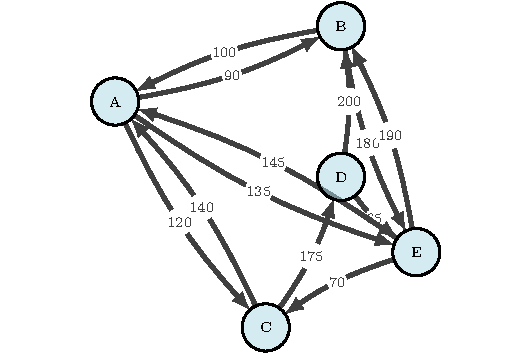
\includegraphics[width=12cm]{airline.pdf}
    \caption{Graphe des liaisons entre villes}
    \label{fig:airline}
  \end{center}
\end{figure}

Les itérations de l'algorithme (au départ de A) sont décrites ci-dessous. 

  
\begin{tabular}{c|cccccc}
  & \textbf{A}	&B	&C	&D	&E	& \\
  \hline
  \texttt{pred} &	&A	&A	&	&A	&\\
  \texttt{dist} & 0	&90	&120	&$+\infty$	&135	&\\
\end{tabular}

\begin{tabular}{c|cccccc}
  & \textbf{A}	&\textbf{B}	&C	&D	&E	& \\
  \hline
  \texttt{pred} &	&A	&A	&	&A	&\\
  \texttt{dist} & 0	&90	&120	&$+\infty$	&135	&\\
\end{tabular}

\begin{tabular}{c|cccccc}
  & \textbf{A}	&\textbf{B}	&\textbf{C}	&D	&E	& \\
  \hline
  \texttt{pred} &	&A	&A	&C	&A	&\\
  \texttt{dist} & 0	&90	&120	&295	&135	&\\
\end{tabular}

\begin{tabular}{c|cccccc}
  & \textbf{A}	&\textbf{B}	&\textbf{C}	&D	&\textbf{E}	& \\
  \hline
  \texttt{pred} &	&A	&A	&C	&A	&\\
  \texttt{dist} & 0	&90	&120	&295	&135	&\\
\end{tabular}

\begin{tabular}{c|cccccc}
  & \textbf{A}	&\textbf{B}	&\textbf{C}	&\textbf{D}	&\textbf{E}	& \\
  \hline
  \texttt{pred} &	&A	&A	&C	&A	&\\
  \texttt{dist} & 0	&90	&120	&295	&135	&\\  
\end{tabular}

Pour obtenir un distancier, ce n'est pas la méthode la plus efficace car il faudrait recommencer au départ de chaque sommet, il vaut mieux utiliser l'algorithme de Bellman dans sa version matricielle qui donnera bien le résultat escompté. Alternativement,on peut utiliser l'algorithme de Roy-Warshall vu en TD. 

La matrice d'adjacence pondérée s'écrit ainsi :

\begin{equation}
  M = \begin{pmatrix}
    0 & 90 & 120 & +\infty & 135 \\
    100 & 0 & +\infty & +\infty & 180 \\
    140 & +\infty & 0 & 175 & +\infty \\
    +\infty & 200 & +\infty & 0 & 95 \\
    145 & 190 & 70 & +\infty & 0 \\
  \end{pmatrix}
\end{equation}

Les itérations de l'algorithme de Bellman s'écrivent ensuite comme suit.

$$
M_1 =
\begin{pmatrix}
  0& 90& 120& +\infty& 135\\
  100& 0& 220& +\infty& 180\\
  140& 230& 0& 175& 275\\
  +\infty& 200& +\infty& 0& 65\\
  145& 190& 70& +\infty& 0\\
  \end{pmatrix}
$$

$$
M_2 =
\begin{pmatrix}
  0& 90& 120& +\infty& 135\\
  100& 0& 220& +\infty& 180\\
  140& 230& 0& 175& 275\\
  300& 200& 420& 0& 65\\
  145& 190& 70& +\infty& 0\\
  \end{pmatrix}
$$

$$
M_3 = 
\begin{pmatrix}
  0& 90& 120& 295& 135\\
  100& 0& 220& 395& 180\\
  140& 230& 0& 175& 275\\
  300& 200& 420& 0& 65\\
  145& 190& 70& 245& 0\\
  \end{pmatrix}
$$

$$
M_4 = 
\begin{pmatrix}
  0& 90& 120& 295& 135\\
  100& 0& 220& 395& 180\\
  140& 230& 0& 175& 240\\
  300& 200& 420& 0& 65\\
  145& 190& 70& 245& 0\\
  \end{pmatrix}
$$

$$
M_5 = 
\begin{pmatrix}
  0& 90& 120& 295& 135\\
  100& 0& 220& 395& 180\\
  140& 230& 0& 175& 240\\
  210& 200& 135& 0& 65\\
  145& 190& 70& 245& 0\\
  \end{pmatrix}
  $$

Pour tenir compte de la durée des escales en un sommet du graphe, il suffit d'ajouter un sommet fictif et d'y ajouter un arc avec une pondération d'une heure. 

\section{Débit réseau}

On part du graphe à flot nul. 


\begin{figure}[h]
\begin{center}
	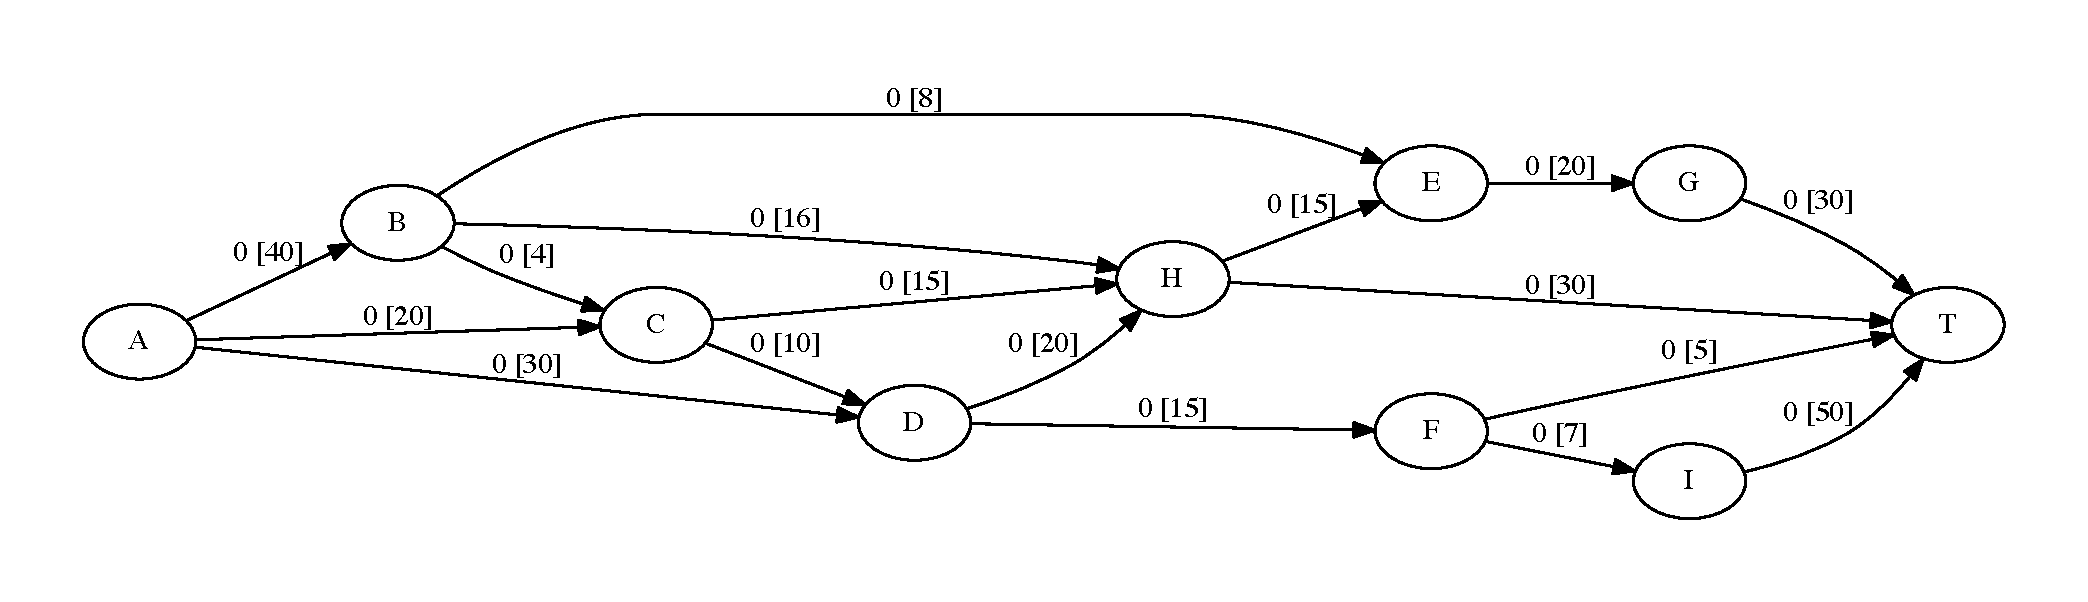
\includegraphics[width=\textwidth]{figs/reseau.pdf}
	\caption{Flot initial nul}
	\label{fig:res:0}
\end{center}
\end{figure}

On choisit une première chaîne augmentante : A-B-H-T, on peut augmenter le flot du minimum des capacités, soit 16, ce qui donne le graphe suivant.

\begin{figure}[h]
\begin{center}
	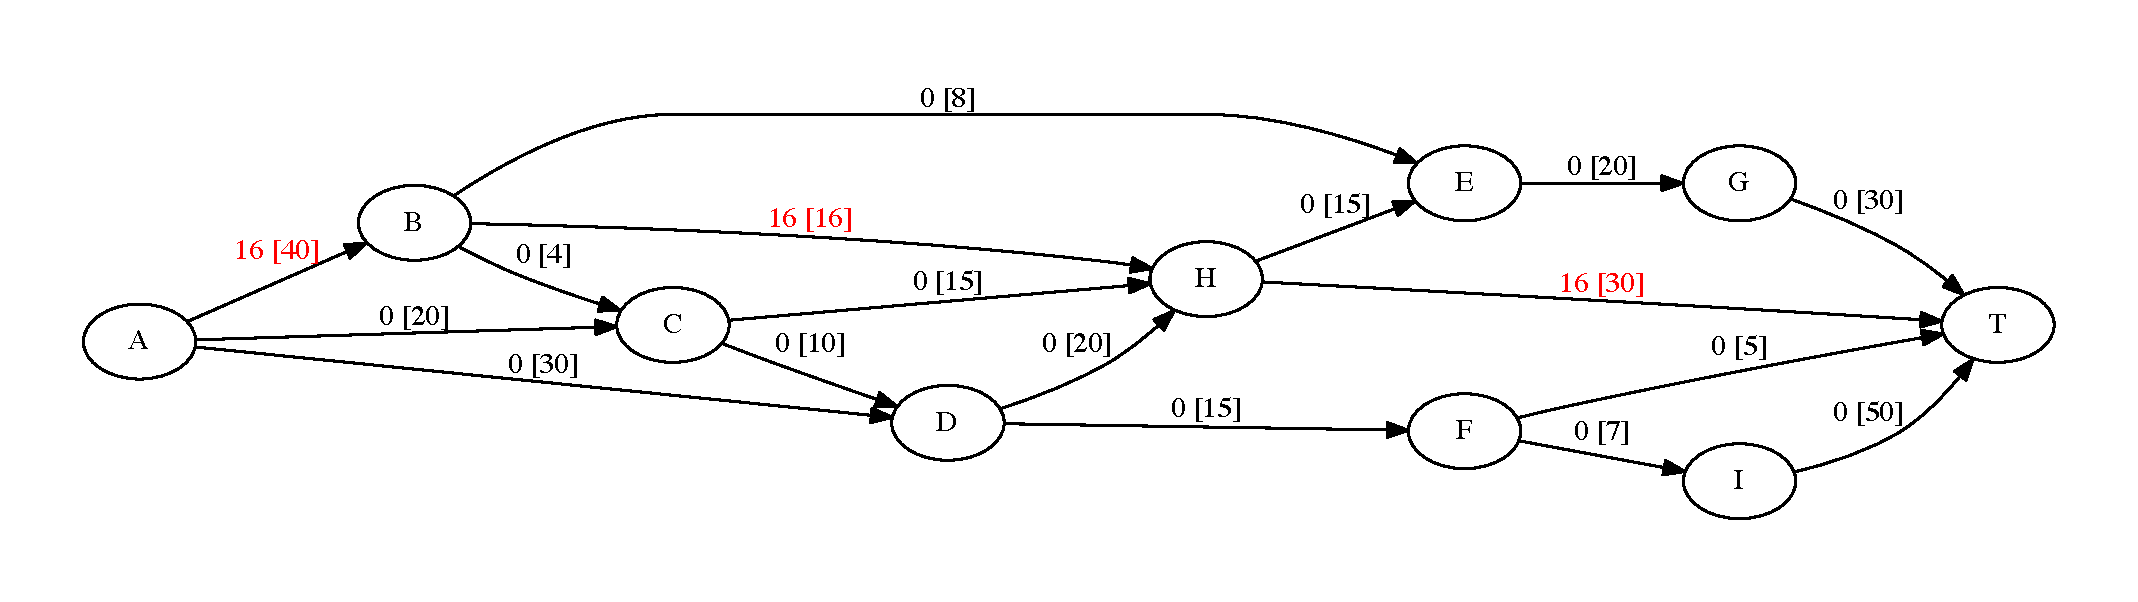
\includegraphics[width=\textwidth]{figs/reseau-1.pdf}
	\caption{Première itération}
	\label{fig:res:1}
\end{center}
\end{figure}

On choisit ensuite une seconde chaîne augmentante, A-D-F-I-T qui permet d'augmenter le flot de 7.

\begin{figure}[h]
\begin{center}
	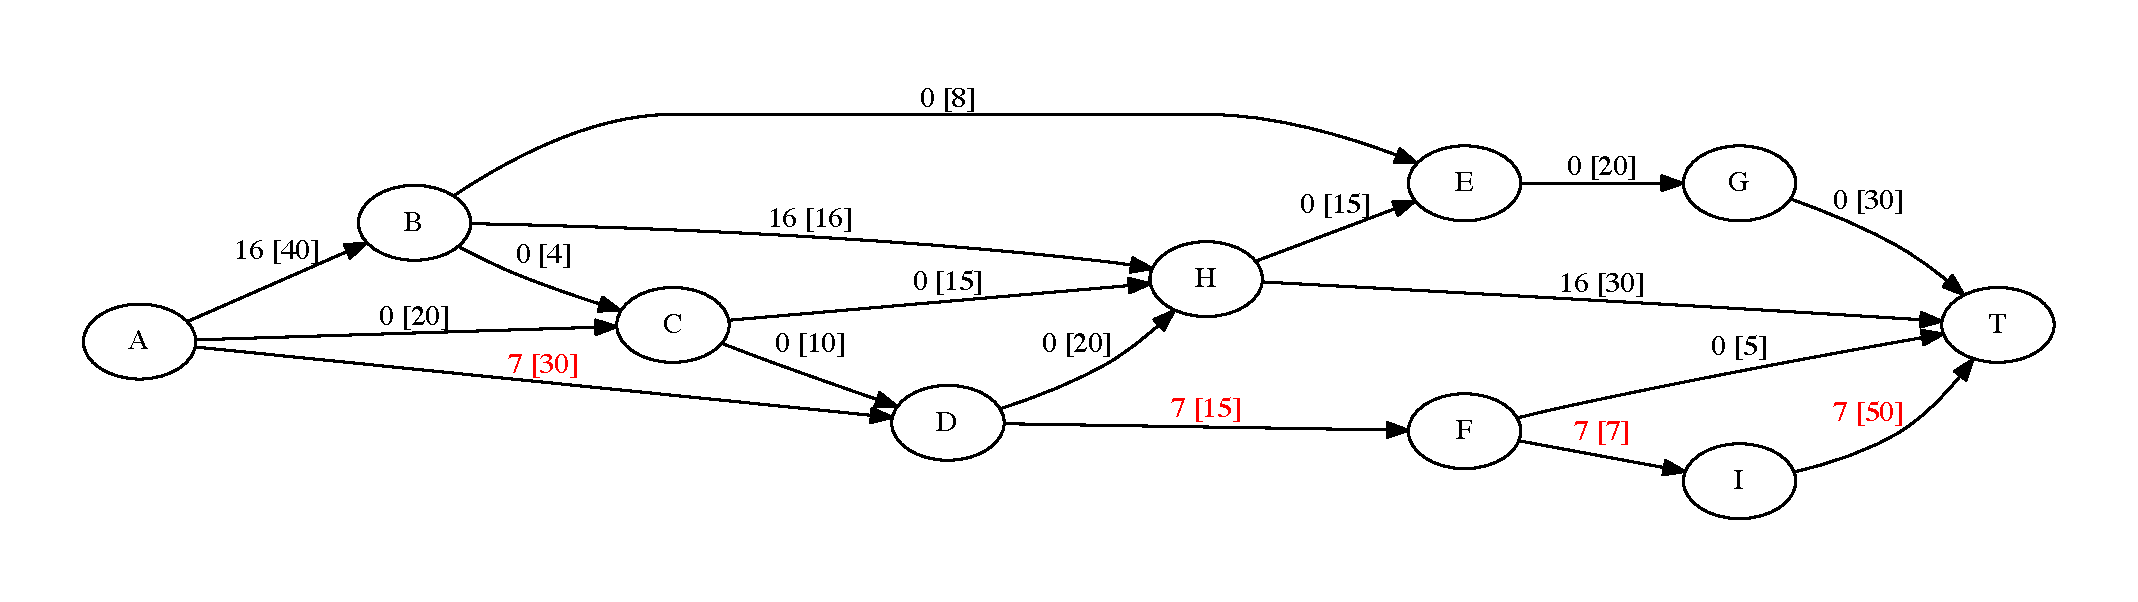
\includegraphics[width=\textwidth]{figs/reseau-2.pdf}
	\caption{Seconde itération}
	\label{fig:res:2}
\end{center}
\end{figure}

Troisième chaîne augmentante : A-B-E-G-T qui permet d'augmenter le flot de 8. 

\begin{figure}[h]
\begin{center}
	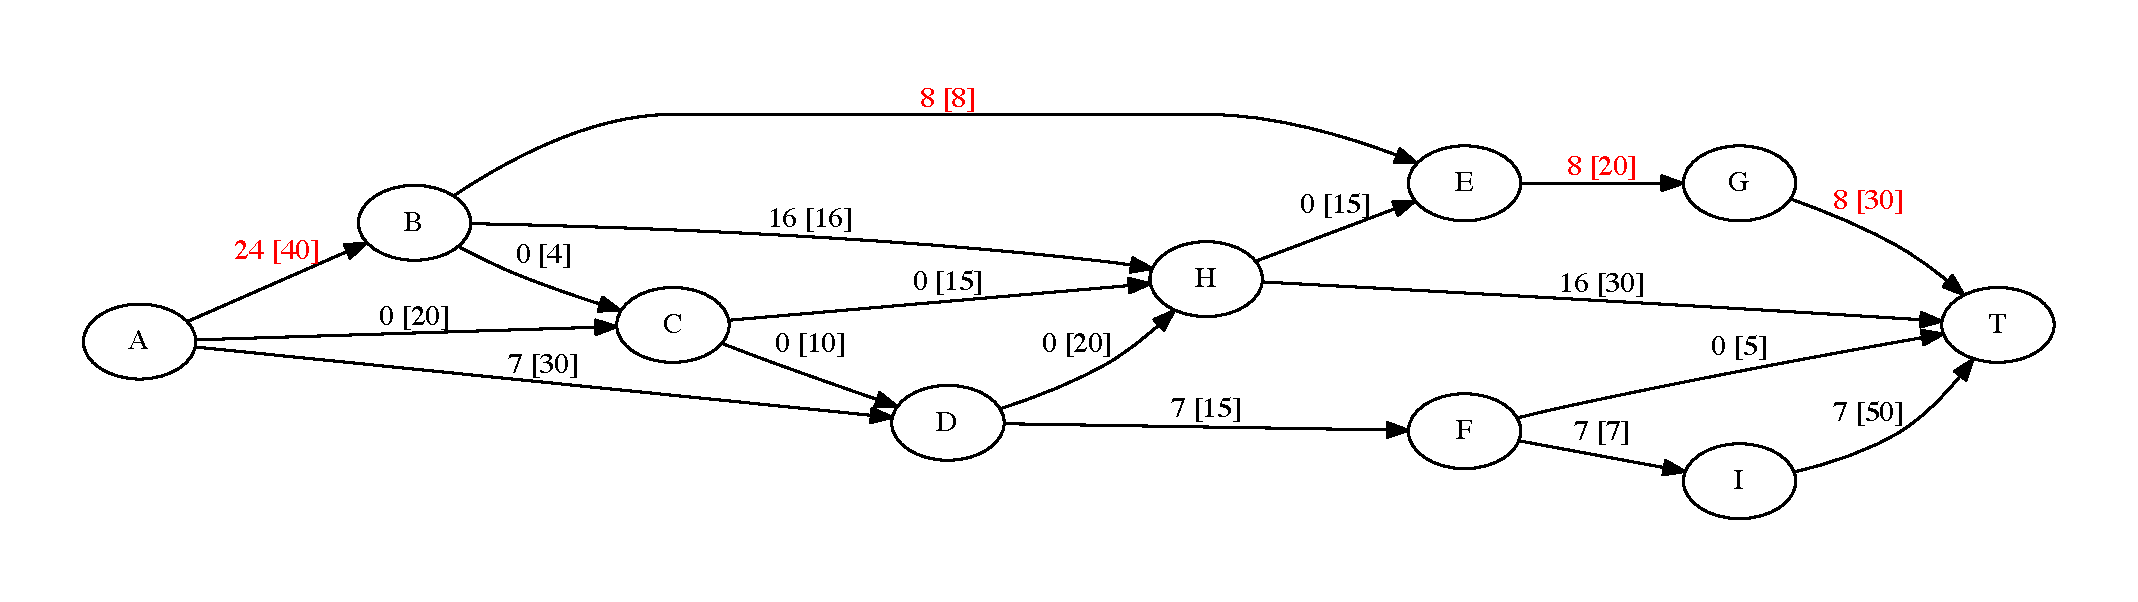
\includegraphics[width=\textwidth]{figs/reseau-3.pdf}
	\caption{Troisième itération}
	\label{fig:res:3}
\end{center}
\end{figure}

Quatrième chaîne augmentante : A-C-H-T qui permet d'augmenter le flot de 14.

\begin{figure}[h]
\begin{center}
	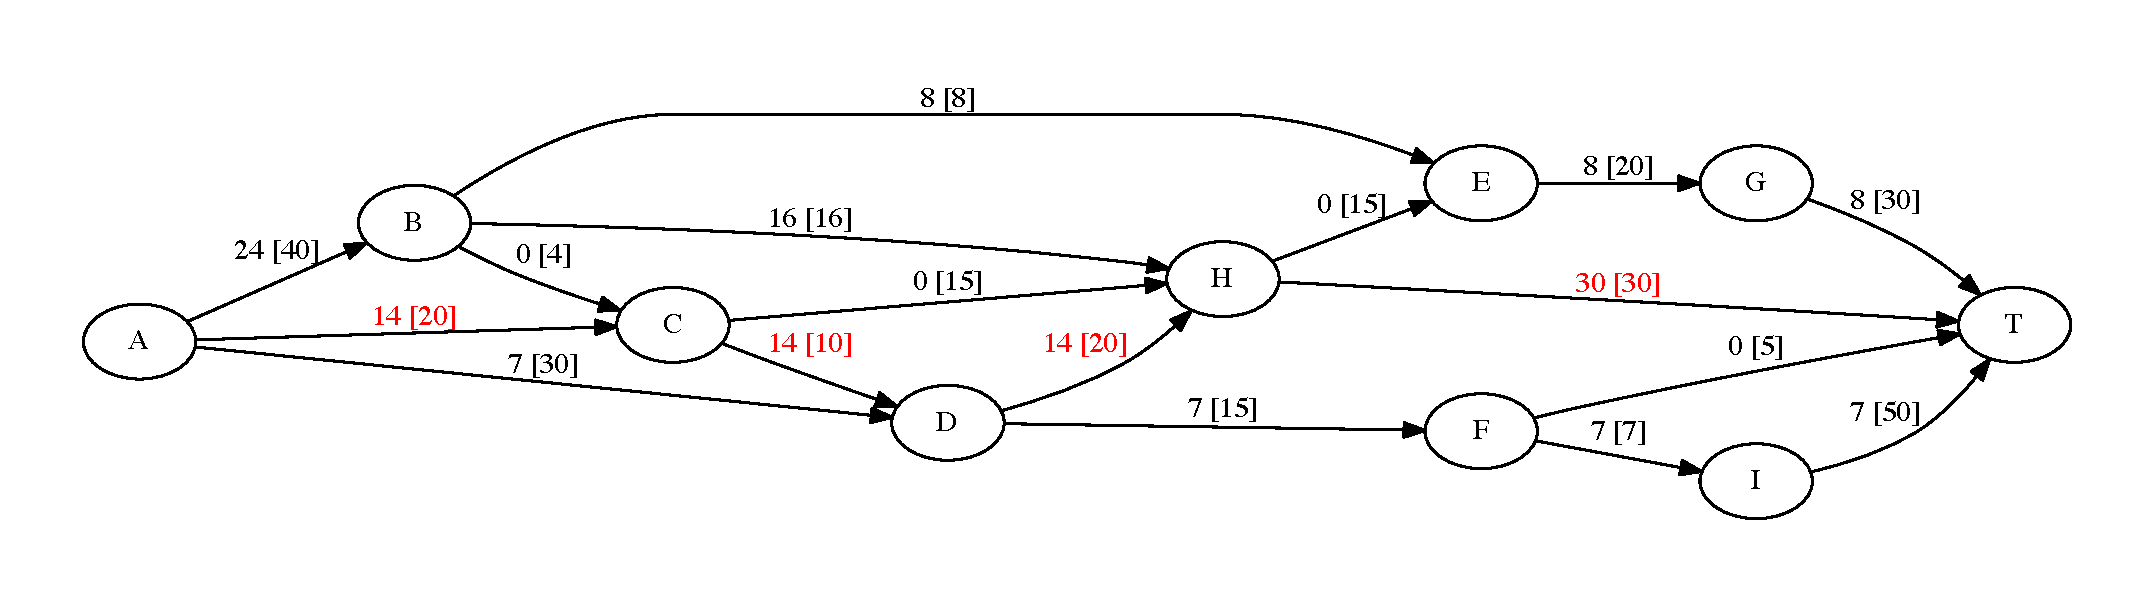
\includegraphics[width=\textwidth]{figs/reseau-4.pdf}
	\caption{Quatrième itération}
	\label{fig:res:4}
\end{center}
\end{figure}

Le graphe devenant moins intuitif, on va appliquer l'algo de marquage compris dans l'algorithme général de Ford \& Fulkerson.

\begin{figure}[h]
\begin{center}
	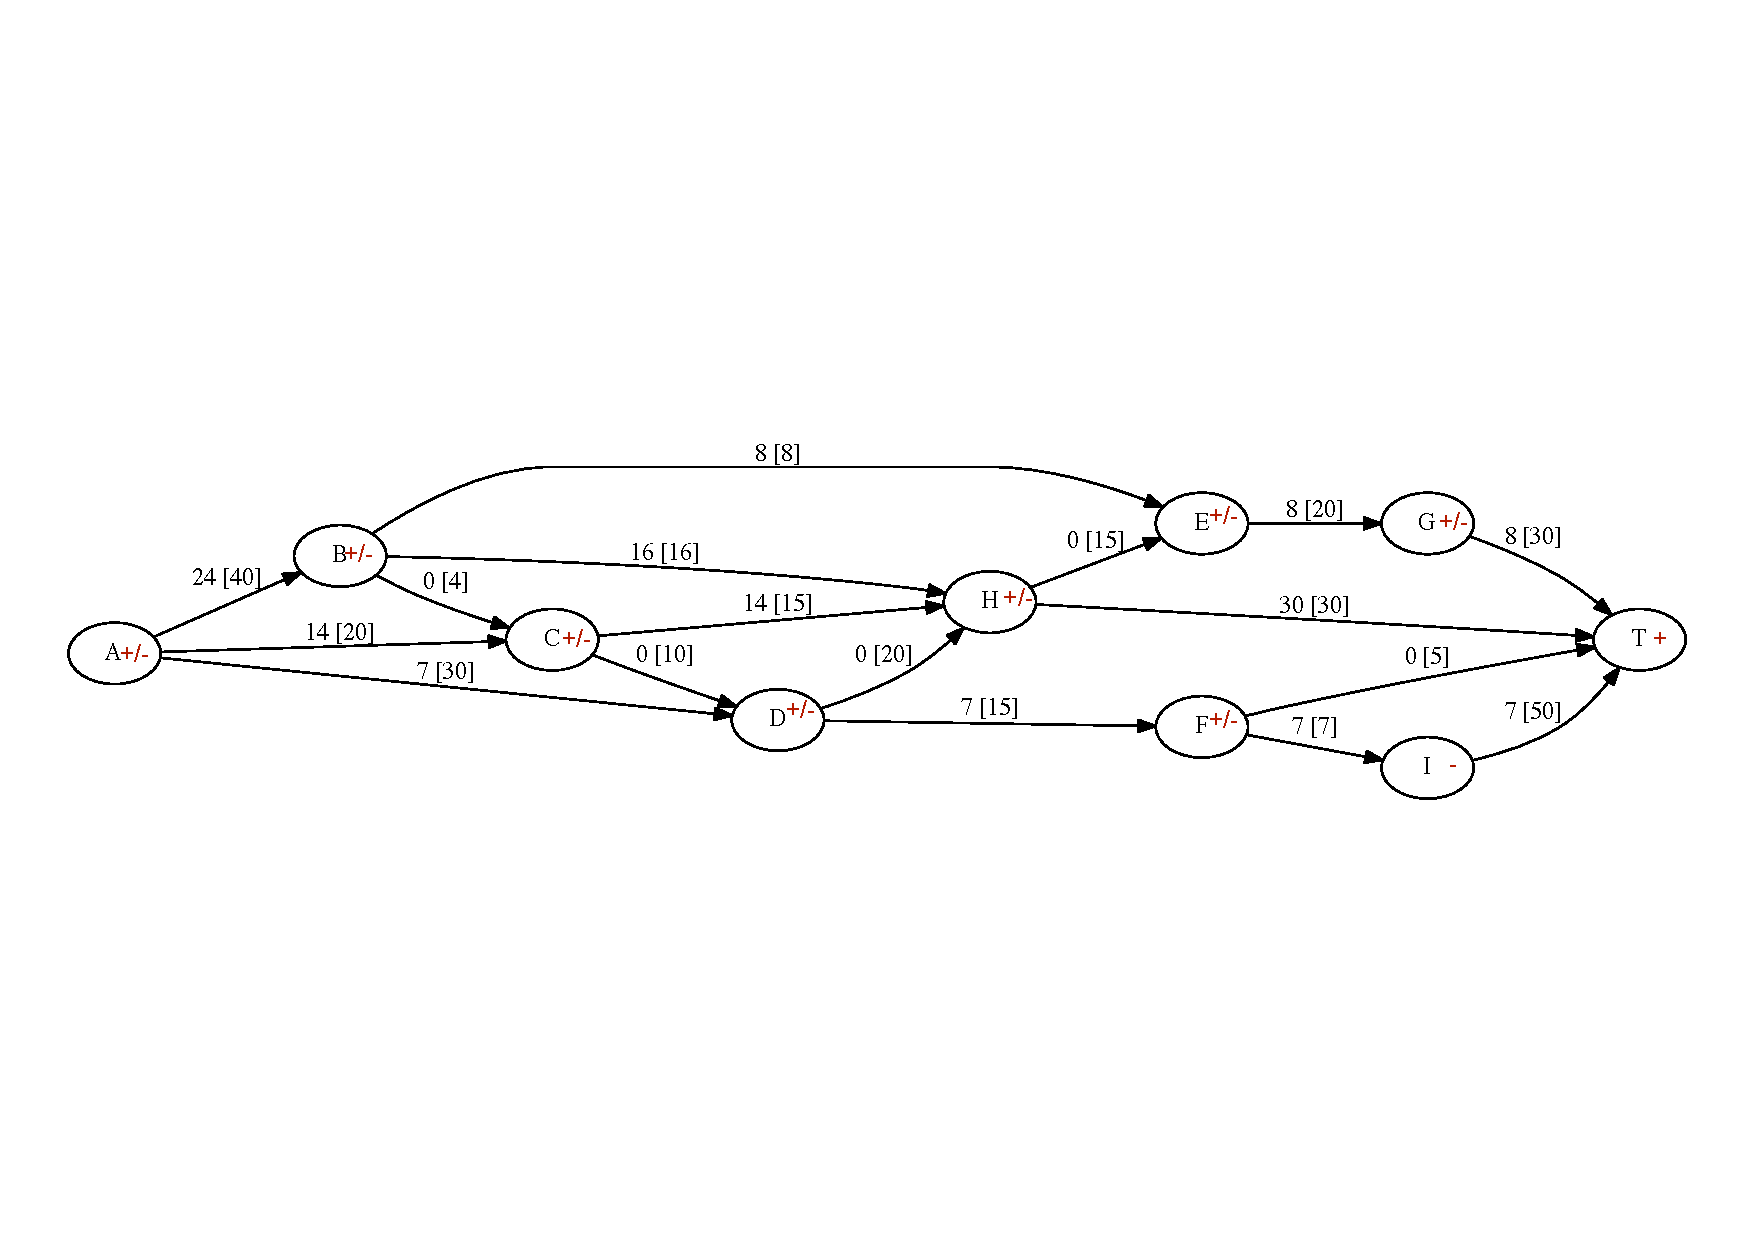
\includegraphics[width=\textwidth]{figs/reseau-4m.pdf}
	\caption{Marquage après la quatrième itération}
	\label{fig:res:4m}
\end{center}
\end{figure}

Ce marquage permet de trouver une chaîne augmentante : A-D-H-E-G-T qui nous permet d'augmenter le flot de 12.

\begin{figure}[h]
\begin{center}
	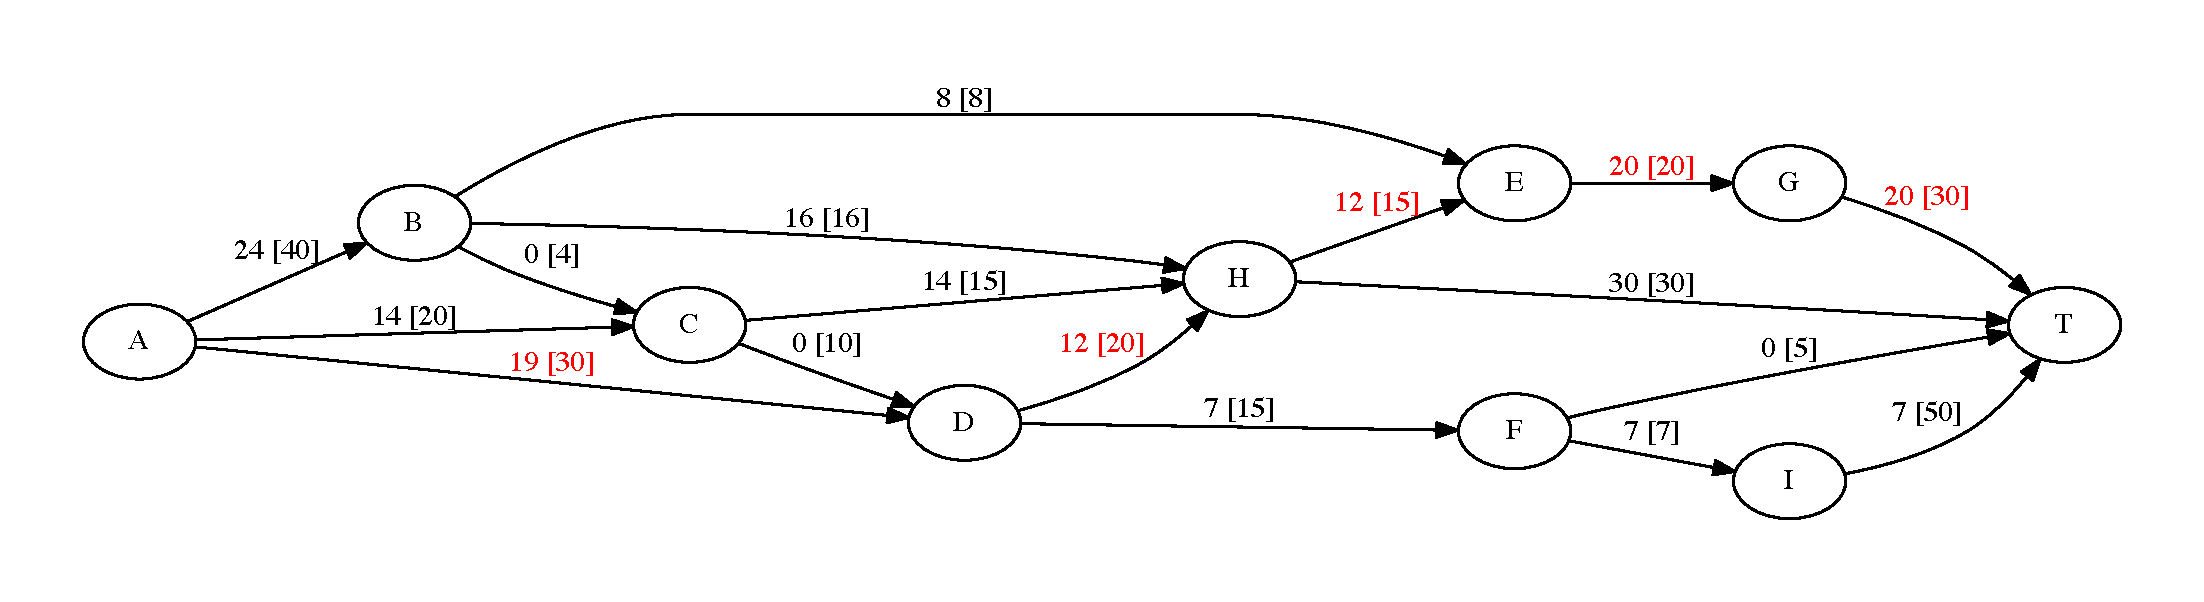
\includegraphics[width=\textwidth]{figs/reseau-5.pdf}
	\caption{Cinquième itération}
	\label{fig:res:5}
\end{center}
\end{figure}

On recommence alors le marquage. 

\begin{figure}[h]
\begin{center}
	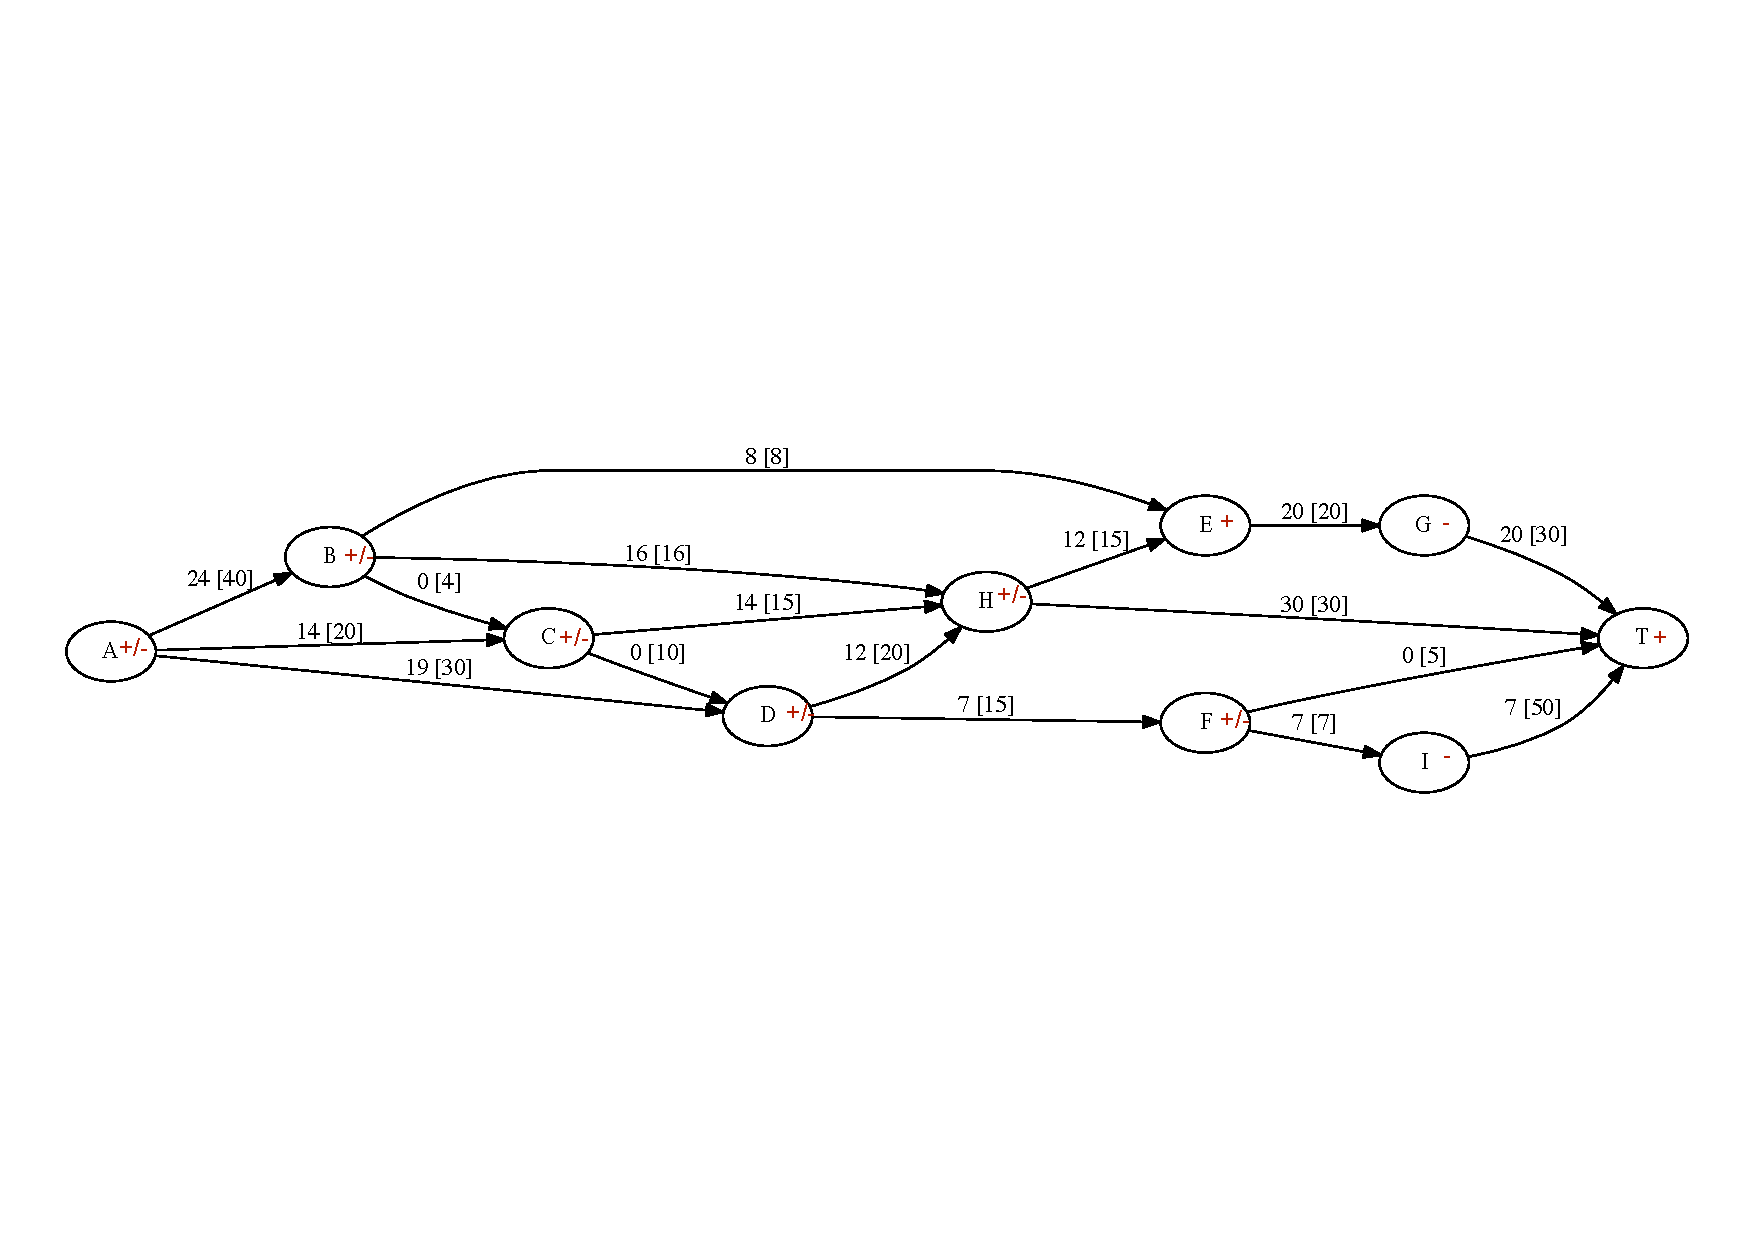
\includegraphics[width=\textwidth]{figs/reseau-5m.pdf}
	\caption{Marquage après la cinquième itération}
	\label{fig:res:5m}
\end{center}
\end{figure}

Celui-ci nous donne une chaîne augmentante A-C-D-F-T qui permet d'augmenter le flot de 5.

\begin{figure}[h]
\begin{center}
	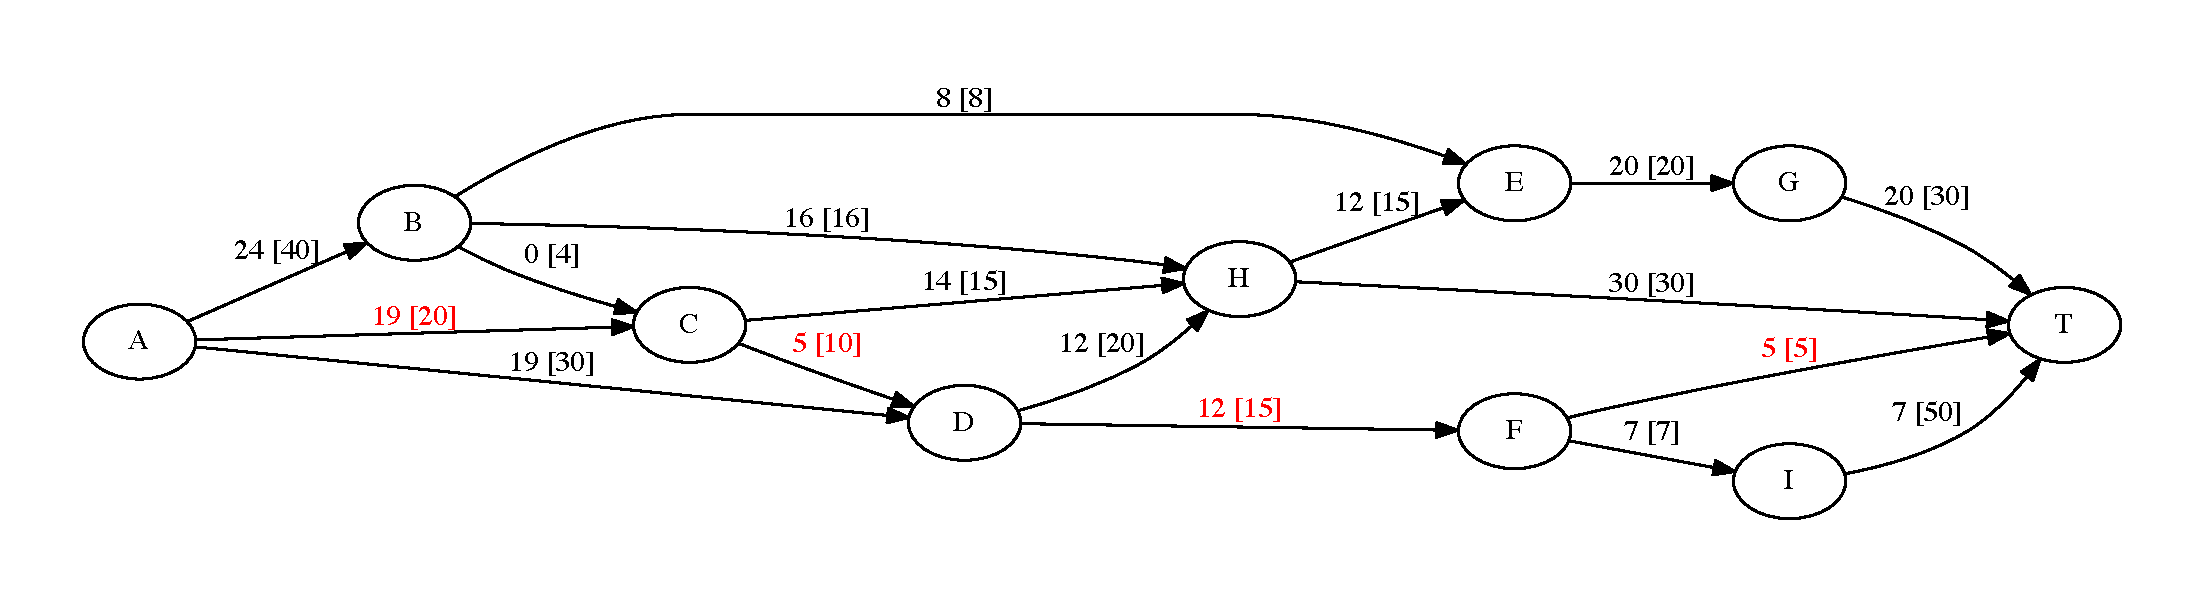
\includegraphics[width=\textwidth]{figs/reseau-6.pdf}
	\caption{Sixième itération}
	\label{fig:res:6}
\end{center}
\end{figure}

On ré-applique l'algorithme de marquage. Le sommet $T$ n'étant pas marqué +, l'algorithme est terminé. On vérifie en traçant la coupe (cf figure), la capacité de celle-ci est de 62, ce qui correspond au flot que nous avons construit. Ouf !

\begin{figure}[h]
\begin{center}
	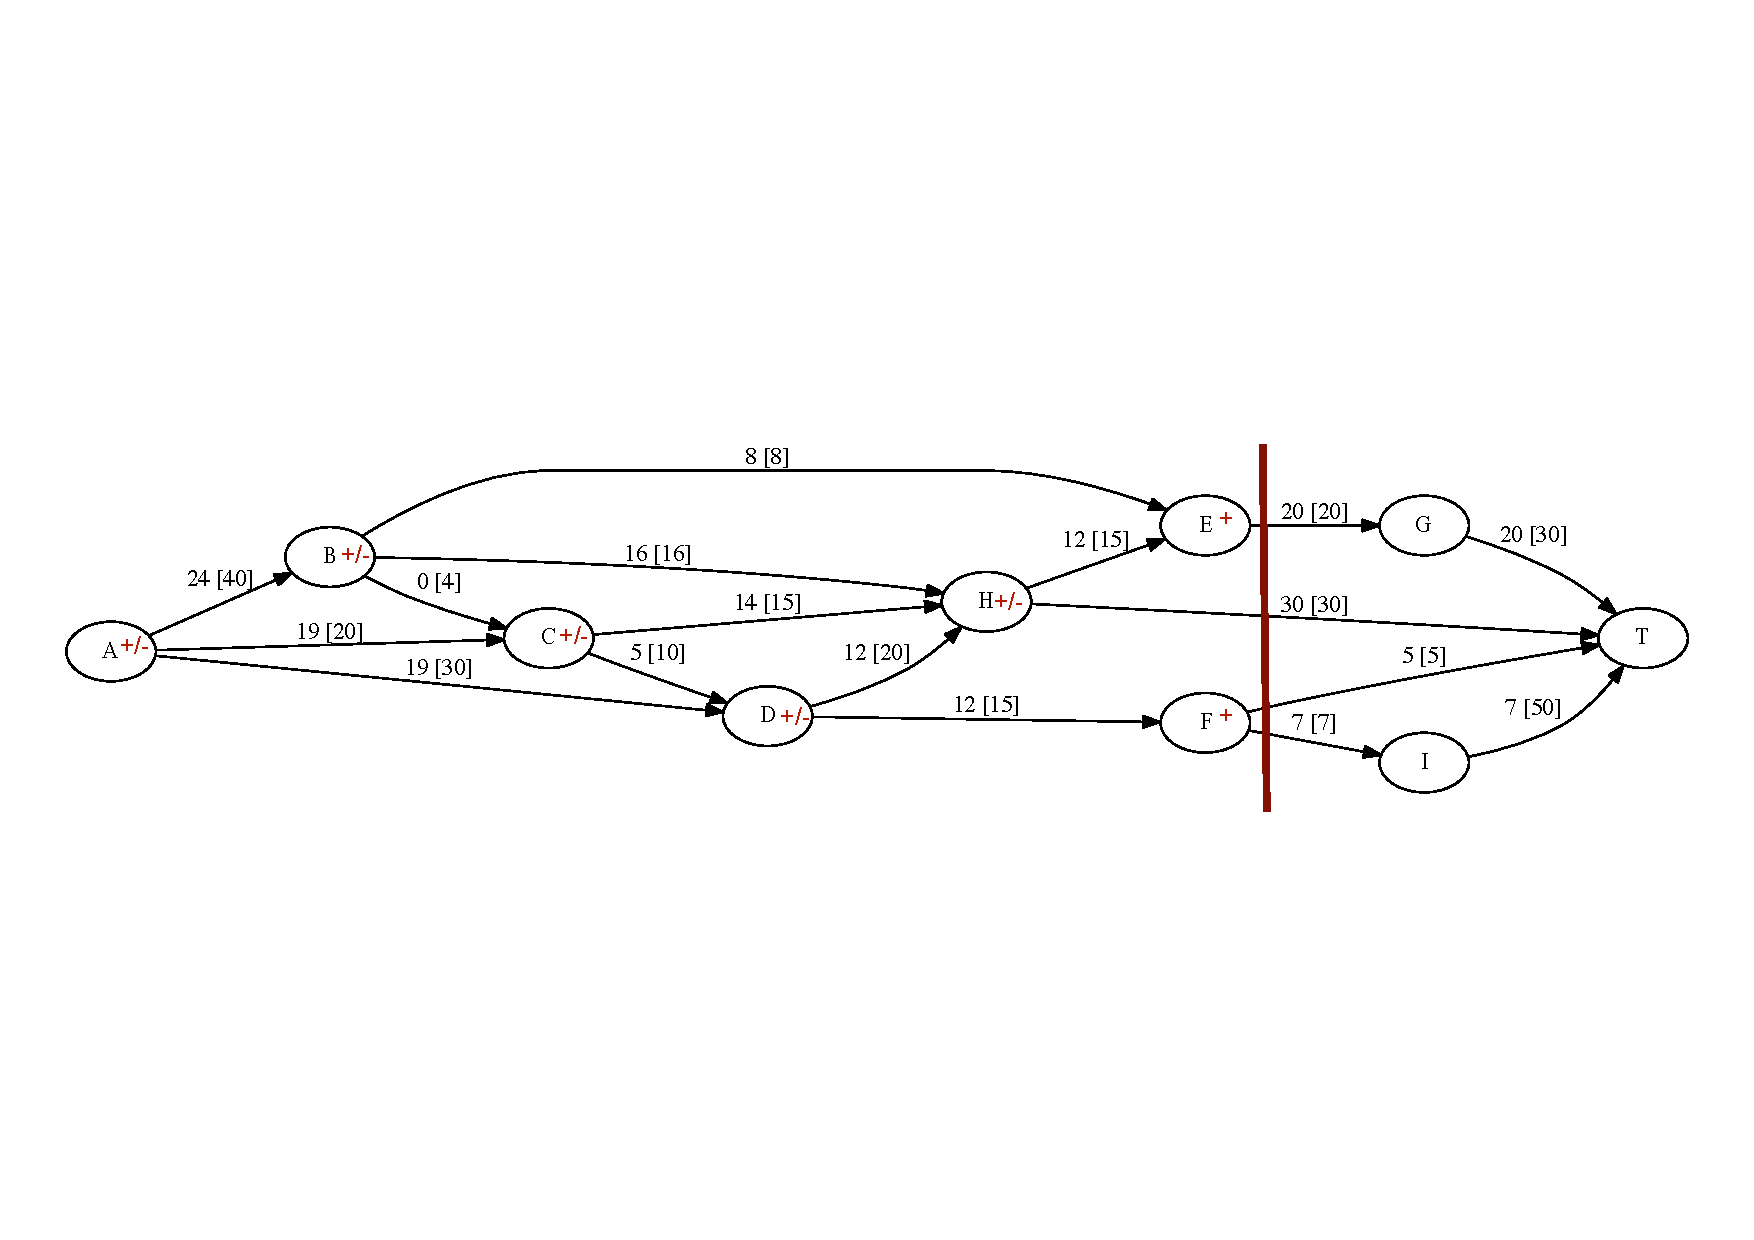
\includegraphics[width=\textwidth]{figs/reseau-6m.pdf}
	\caption{Marquage après la sixième itération}
	\label{fig:res:6m}
\end{center}
\end{figure}


\clearpage

\section{Acheminement de passagers}

Le graphe se construit en considérant chaque ville à différents moment : jeudi matin, jeudi soir, vendredi matin, vendredi soir, et samedi matin. F le samedi soir sera considéré comme le puits du graphe.

On note par ailleurs que le séjour dans une ville la journée n'est pas limité en quantité, on peut donc construire un arc entre une ville le matin et la même ville le soir avec une capacité infinie.

Sur le graphe de la figure~\ref{fig:pass:un}, chaque sommet est nommé à partir de 3 lettres : la première représente la ville (A,  B, C ou F), la seconde le jour (J, V, S) et la troisième le moment de la journée (M, S).

\begin{figure}[h]
\begin{center}
	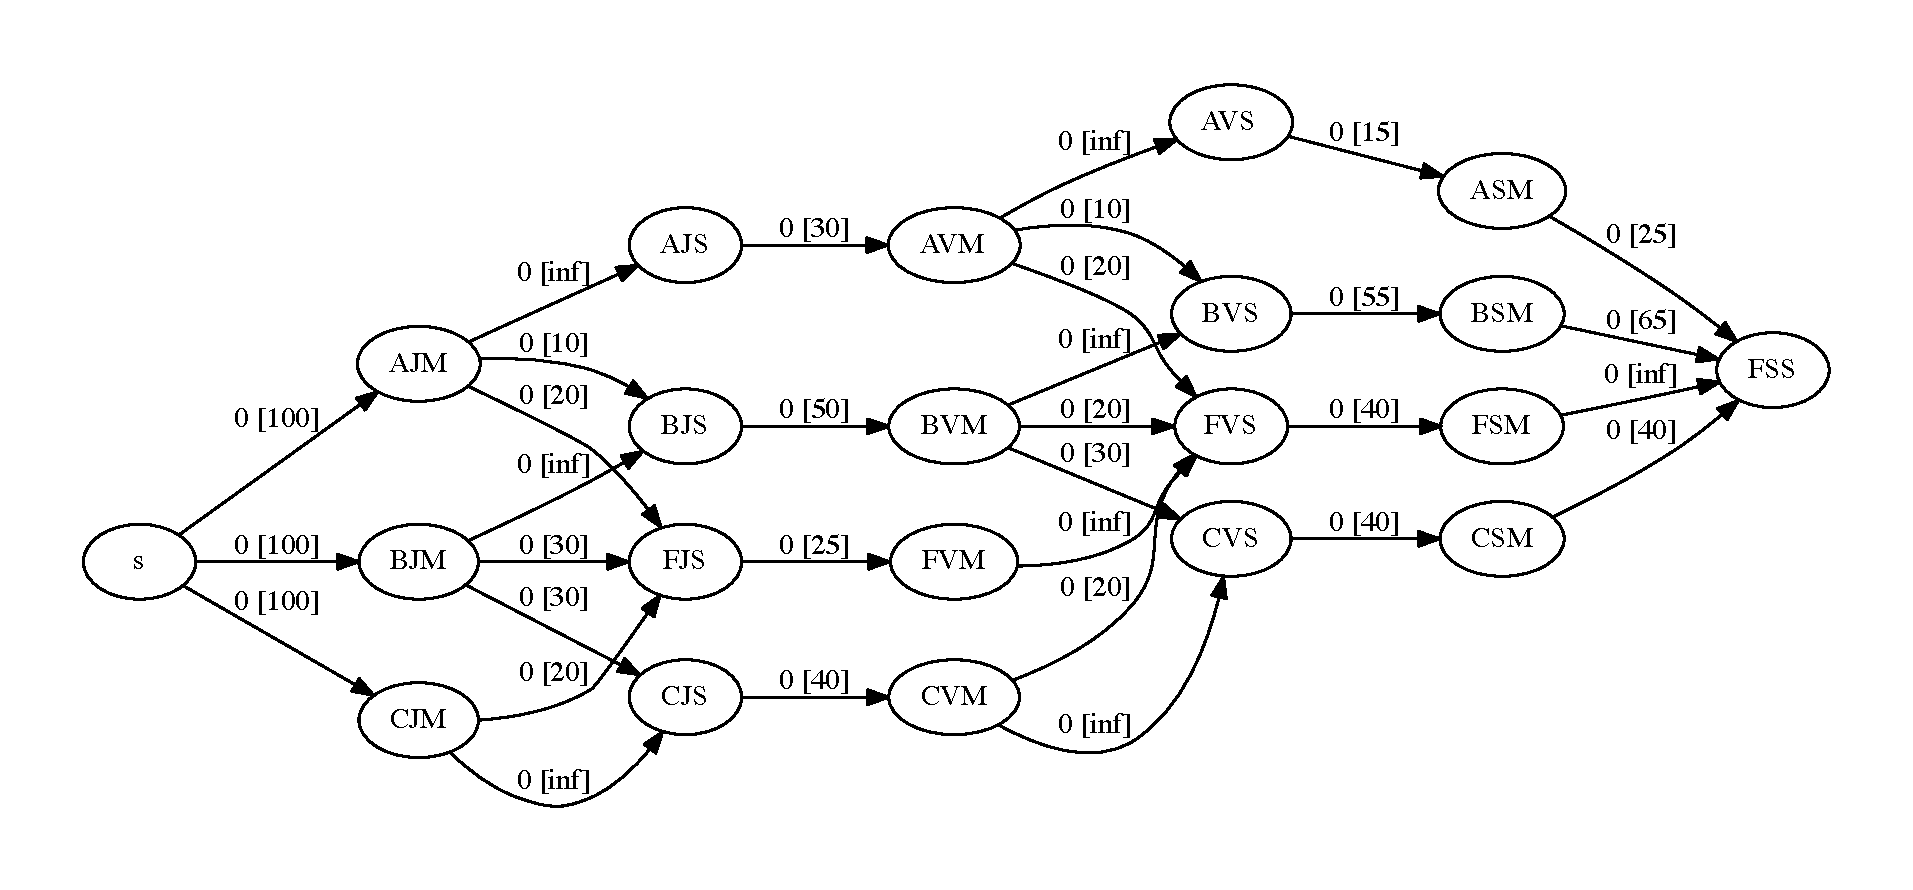
\includegraphics[width=\textwidth]{figs/pass-1.pdf}
	\caption{Graphe initial}
	\label{fig:pass:un}
\end{center}
\end{figure}

Là encore, on peut extraire les chaines augmentantes au fur et mesure en appliquant plus ou moins l'algorithme de marquage.

\begin{enumerate}
\item s-AJM-FJS-FVM-FVS-FSM-FSS : on peut augmenter le flot de 20, voir figure~\ref{fig:pass:deux}
\item s-CJM-CJS-CVM-FVS-FSM-FSS : on peut augmenter le flot de 20, voir figure~\ref{fig:pass:trois}
\item s-BJM-BJS-BVM-BVS-BSM-FSS : on peut augmenter le flot de 50, voir figure~\ref{fig:pass:quatre}
\item s-AJM-AJS-AVM-AVS-ASM-FSS : on peut augmenter le flot de 15, voir figure~\ref{fig:pass:cinq}
\item s-CJM-CJS-CVM-CVS-CSM-FSS : on peut augmenter le flot de 20, voir figure~\ref{fig:pass:six}
\item s-AJM-AJS-AVM-FVS-CVM-CVS-CSM-FSS : on peut augmenter le flot (on a bien ici une \textbf{chaine} augmentante, certains arcs sont utilisés dans le sens puits vers source, le long de l'arc colorié en bleu, on diminue le flot), voir figure~\ref{fig:pass:sept}
\item s-BJM-FJS-FVM-FVS-AVM-BVS-BSM-FSS : on peut augmenter le flot de 5 (toujours en utilisant une \textbf{chaine} augmentante), cf.~\ref{fig:pass:huit}
\end{enumerate}

Il n'existe alors plus de chaine augmentante (figure~\ref{fig:pass:neuf}) : le passage de l'algorithme de marquage ne permettra pas de dépasser le jeudi soir. Cela donne la coupe minimale (en fait la nuit du jeudi au vendredi) pour une valeur de 145. Cela correspond également au flot que nous avons établi et l'algorithme est alors terminé.


\begin{figure}[h]
\begin{center}
	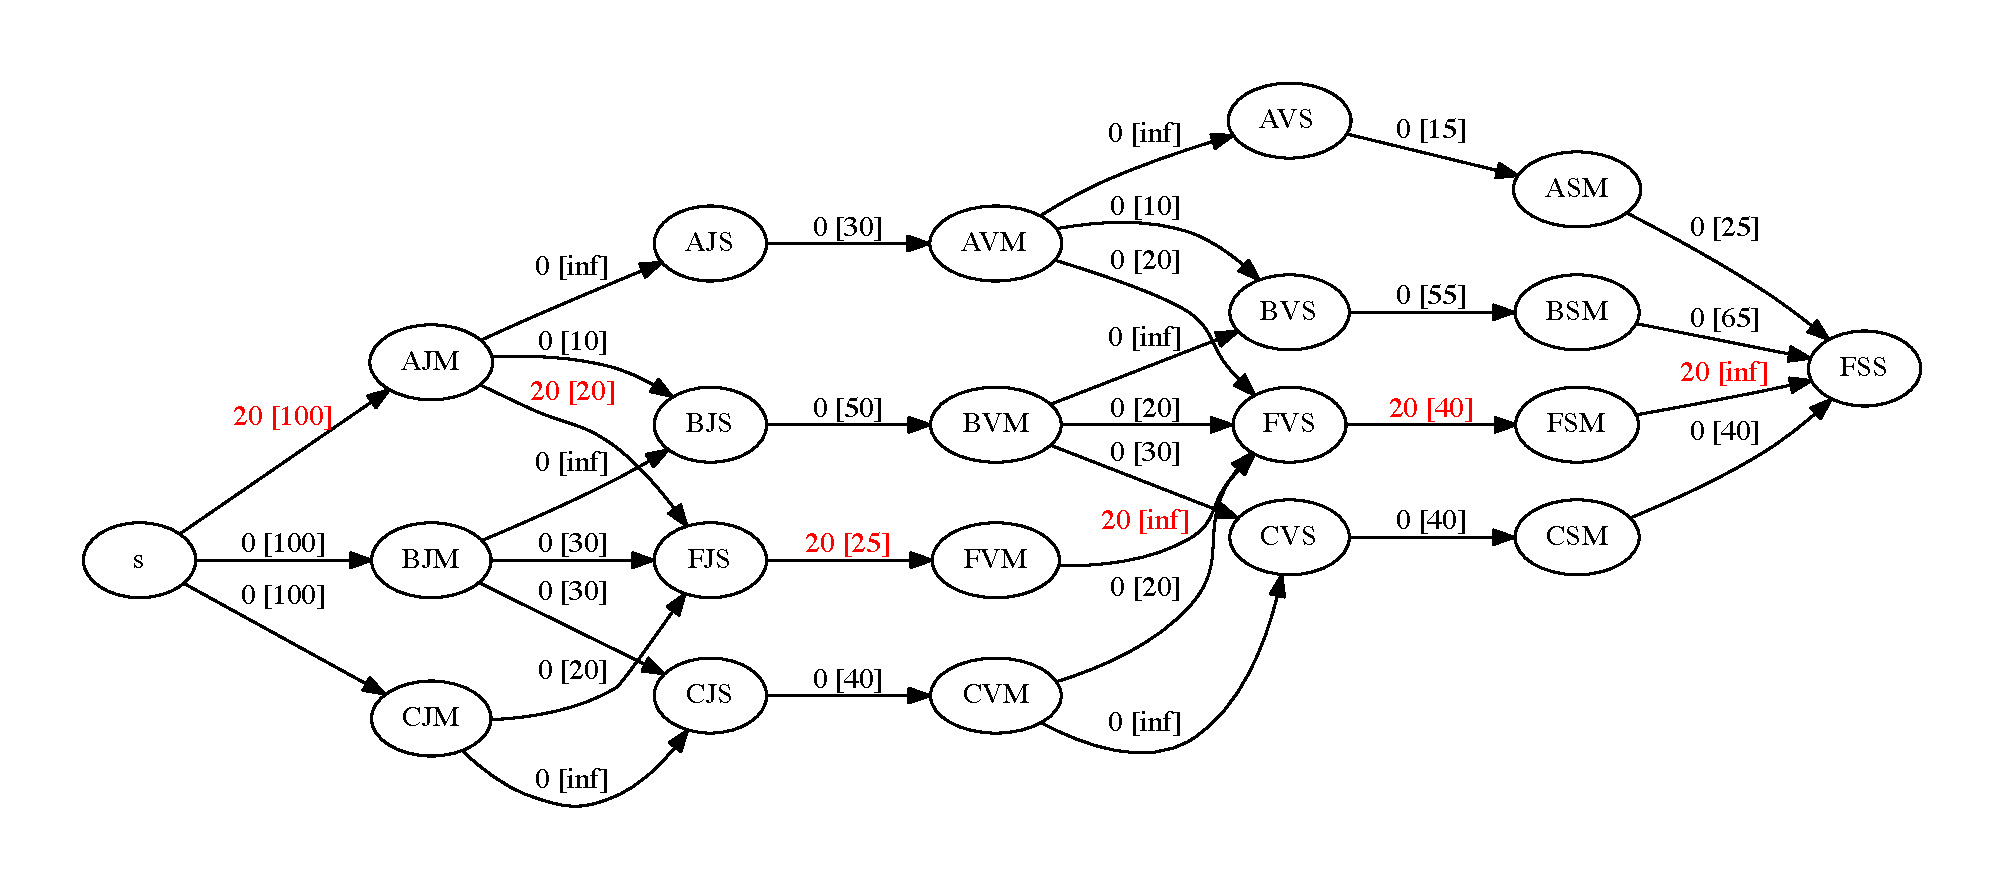
\includegraphics[width=\textwidth]{figs/pass-2.pdf}
	\caption{Première itération}
	\label{fig:pass:deux}
\end{center}
\end{figure}

\begin{figure}[h]
\begin{center}
	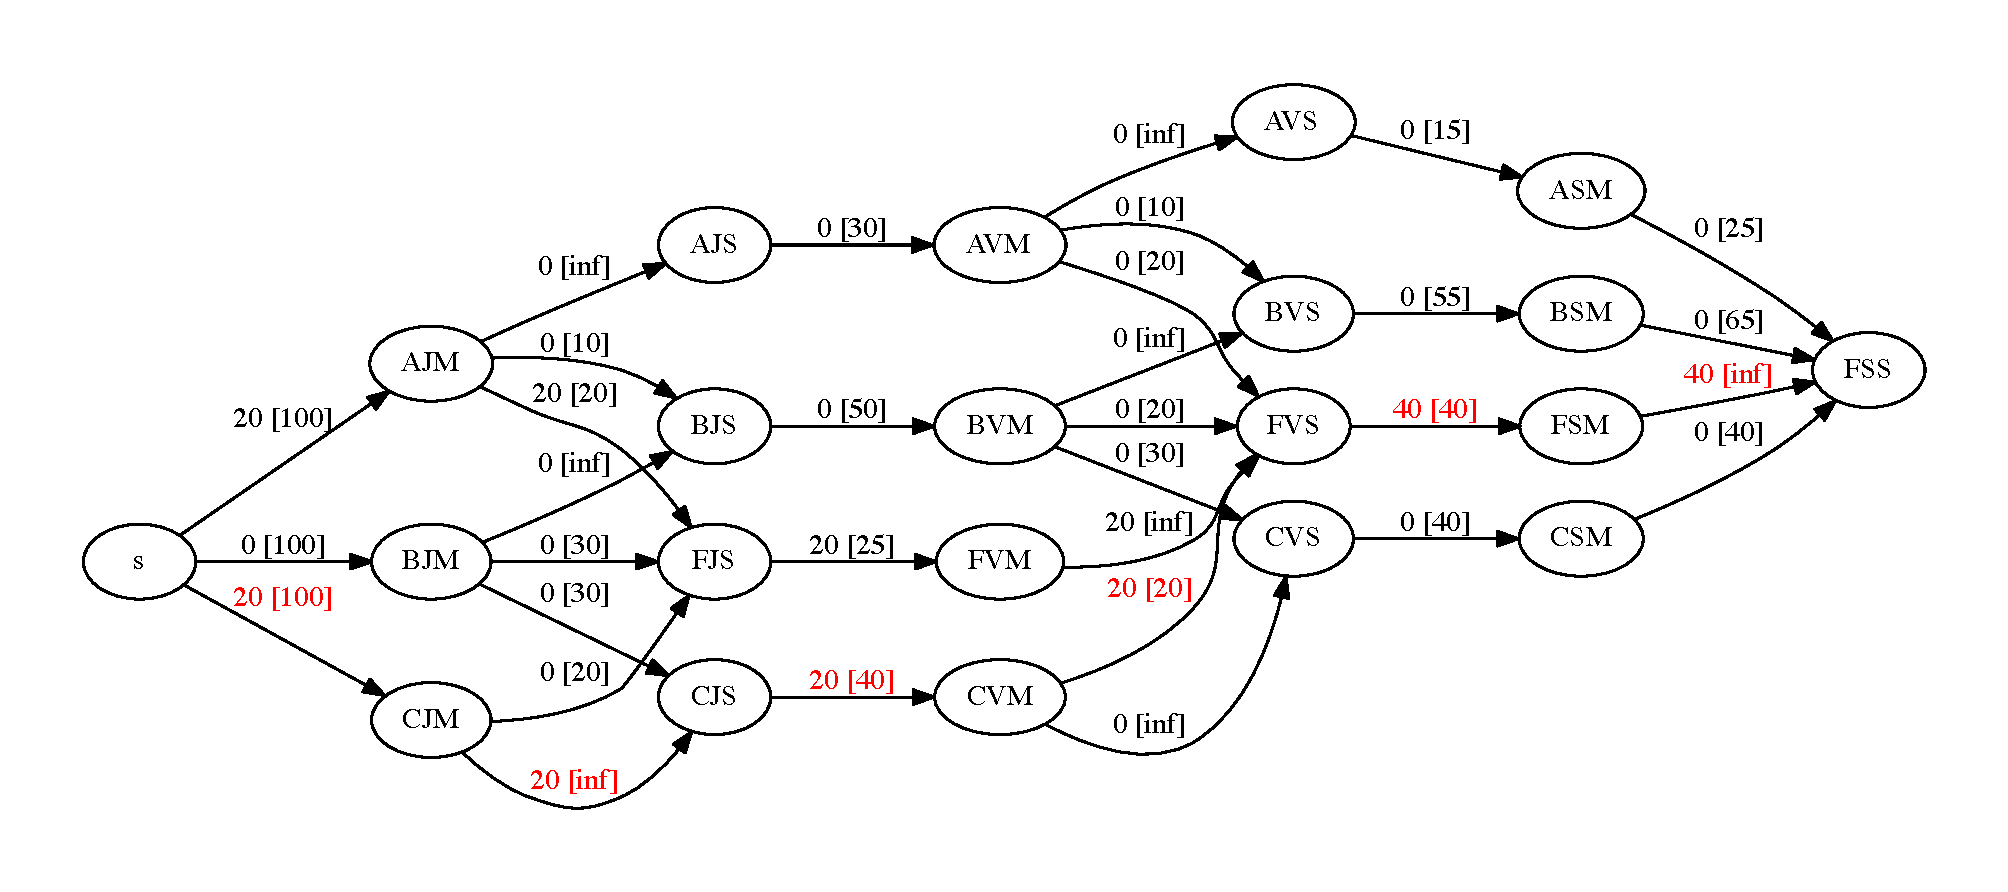
\includegraphics[width=\textwidth]{figs/pass-3.pdf}
	\caption{Seconde itération}
	\label{fig:pass:trois}
\end{center}
\end{figure}

\begin{figure}[h]
\begin{center}
	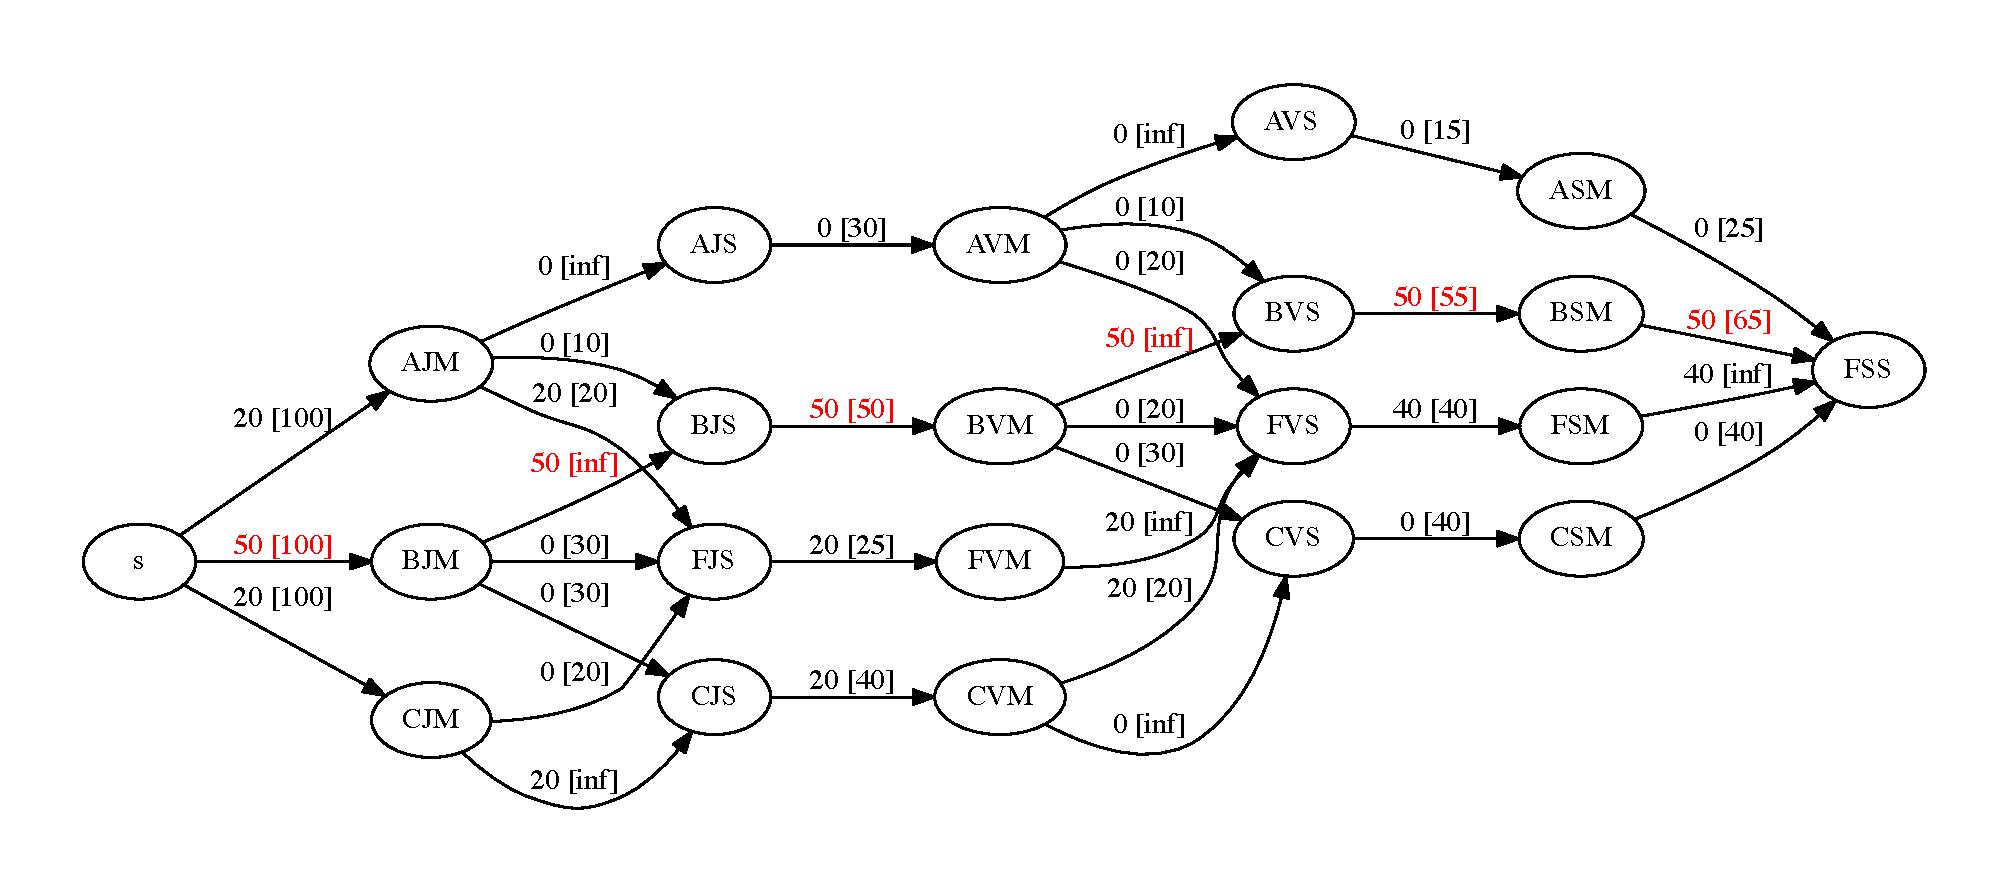
\includegraphics[width=\textwidth]{figs/pass-4.pdf}
	\caption{Troisième itération}
	\label{fig:pass:quatre}
\end{center}
\end{figure}

\begin{figure}[h]
\begin{center}
	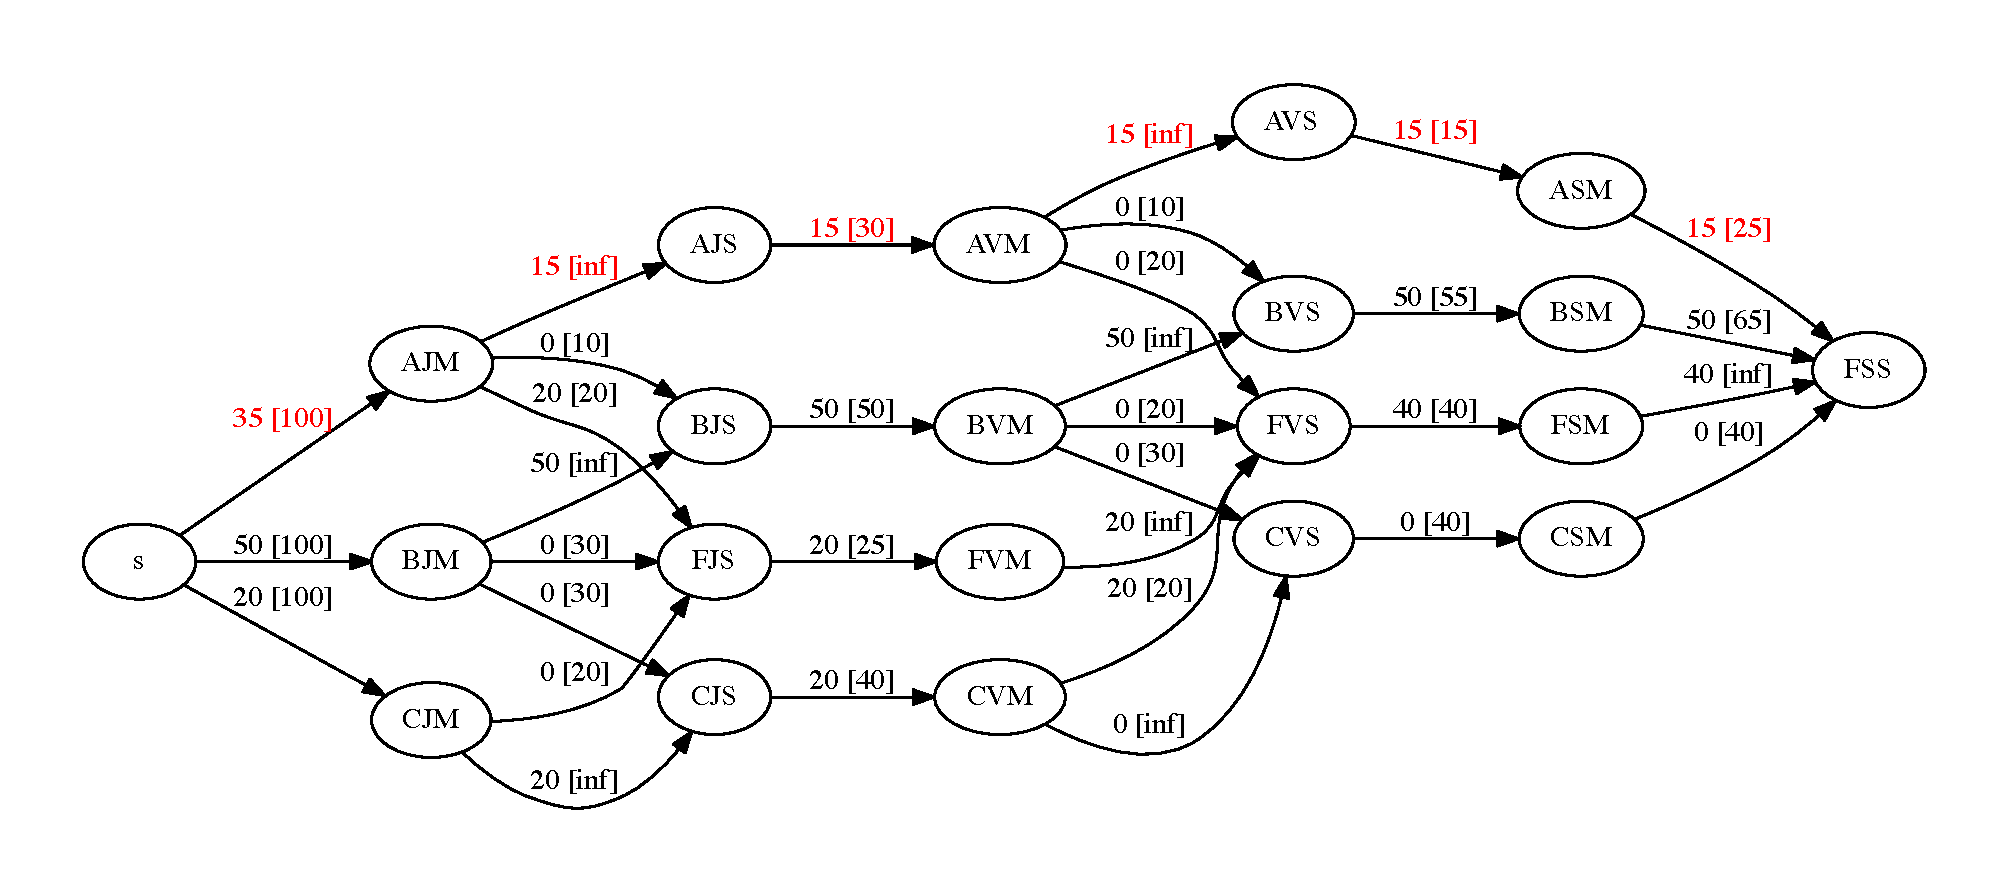
\includegraphics[width=\textwidth]{figs/pass-5.pdf}
	\caption{Quatrième itération}
	\label{fig:pass:cinq}
\end{center}
\end{figure}

\begin{figure}[h]
\begin{center}
	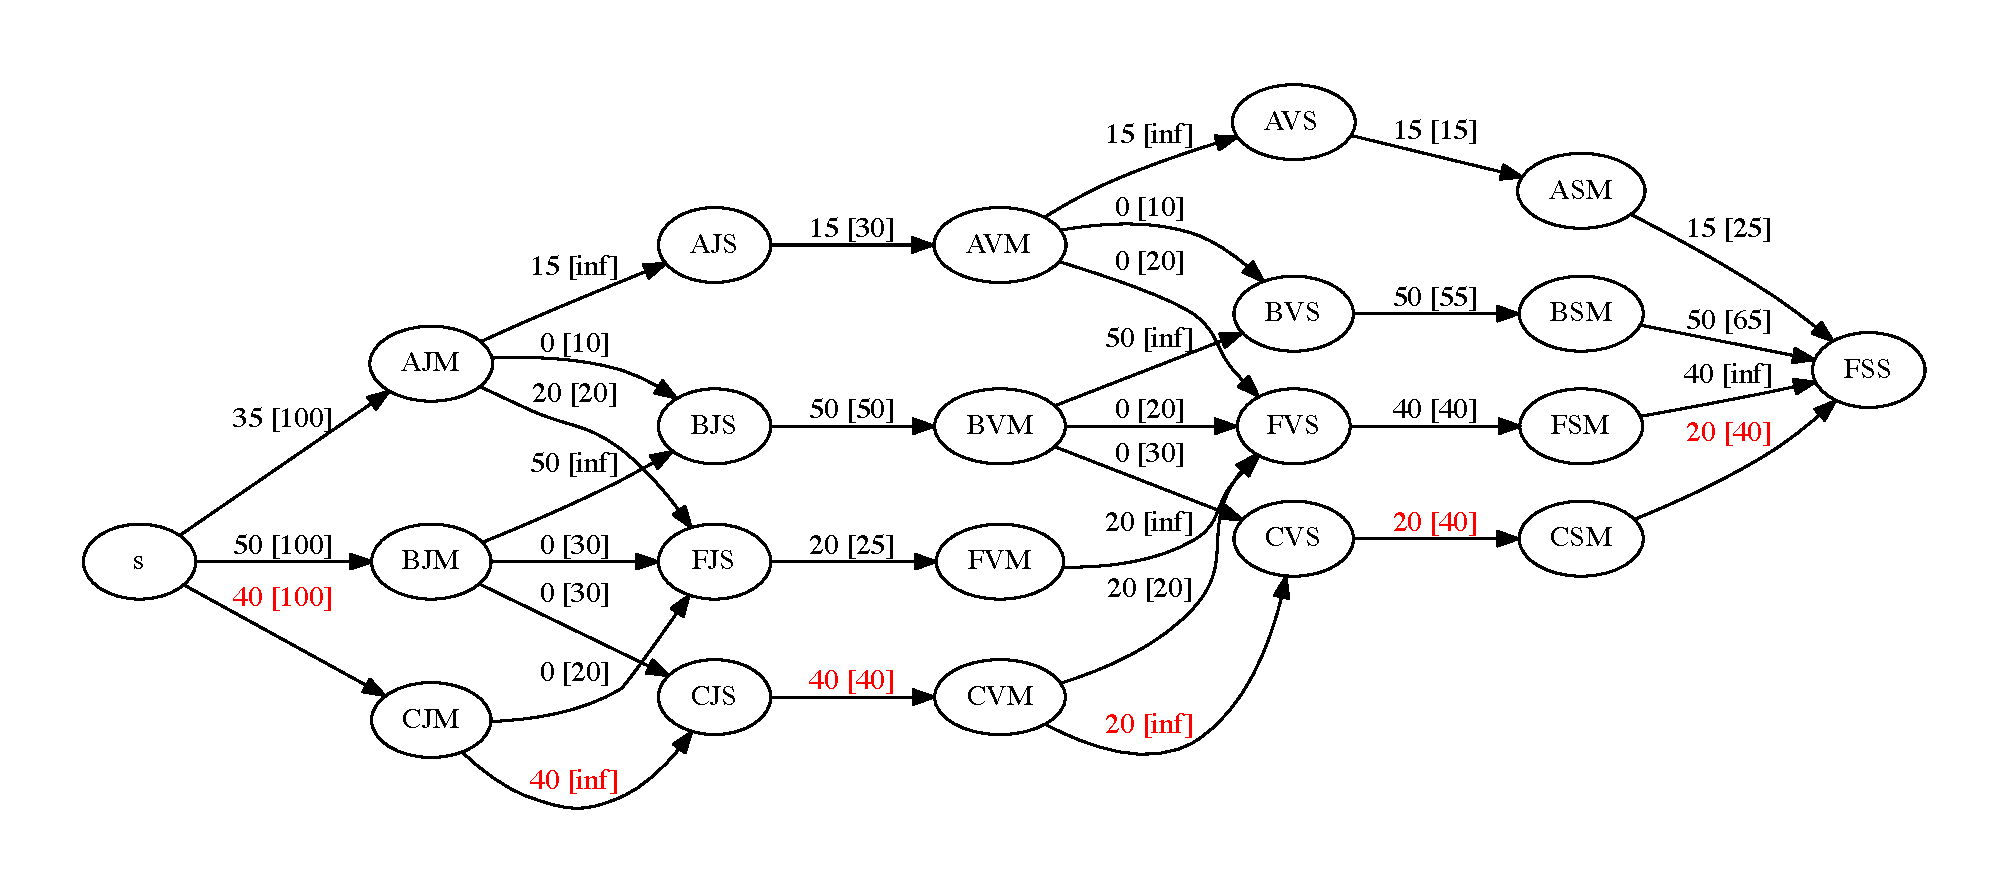
\includegraphics[width=\textwidth]{figs/pass-6.pdf}
	\caption{Cinquième itération}
	\label{fig:pass:six}
\end{center}
\end{figure}

\begin{figure}[h]
\begin{center}
	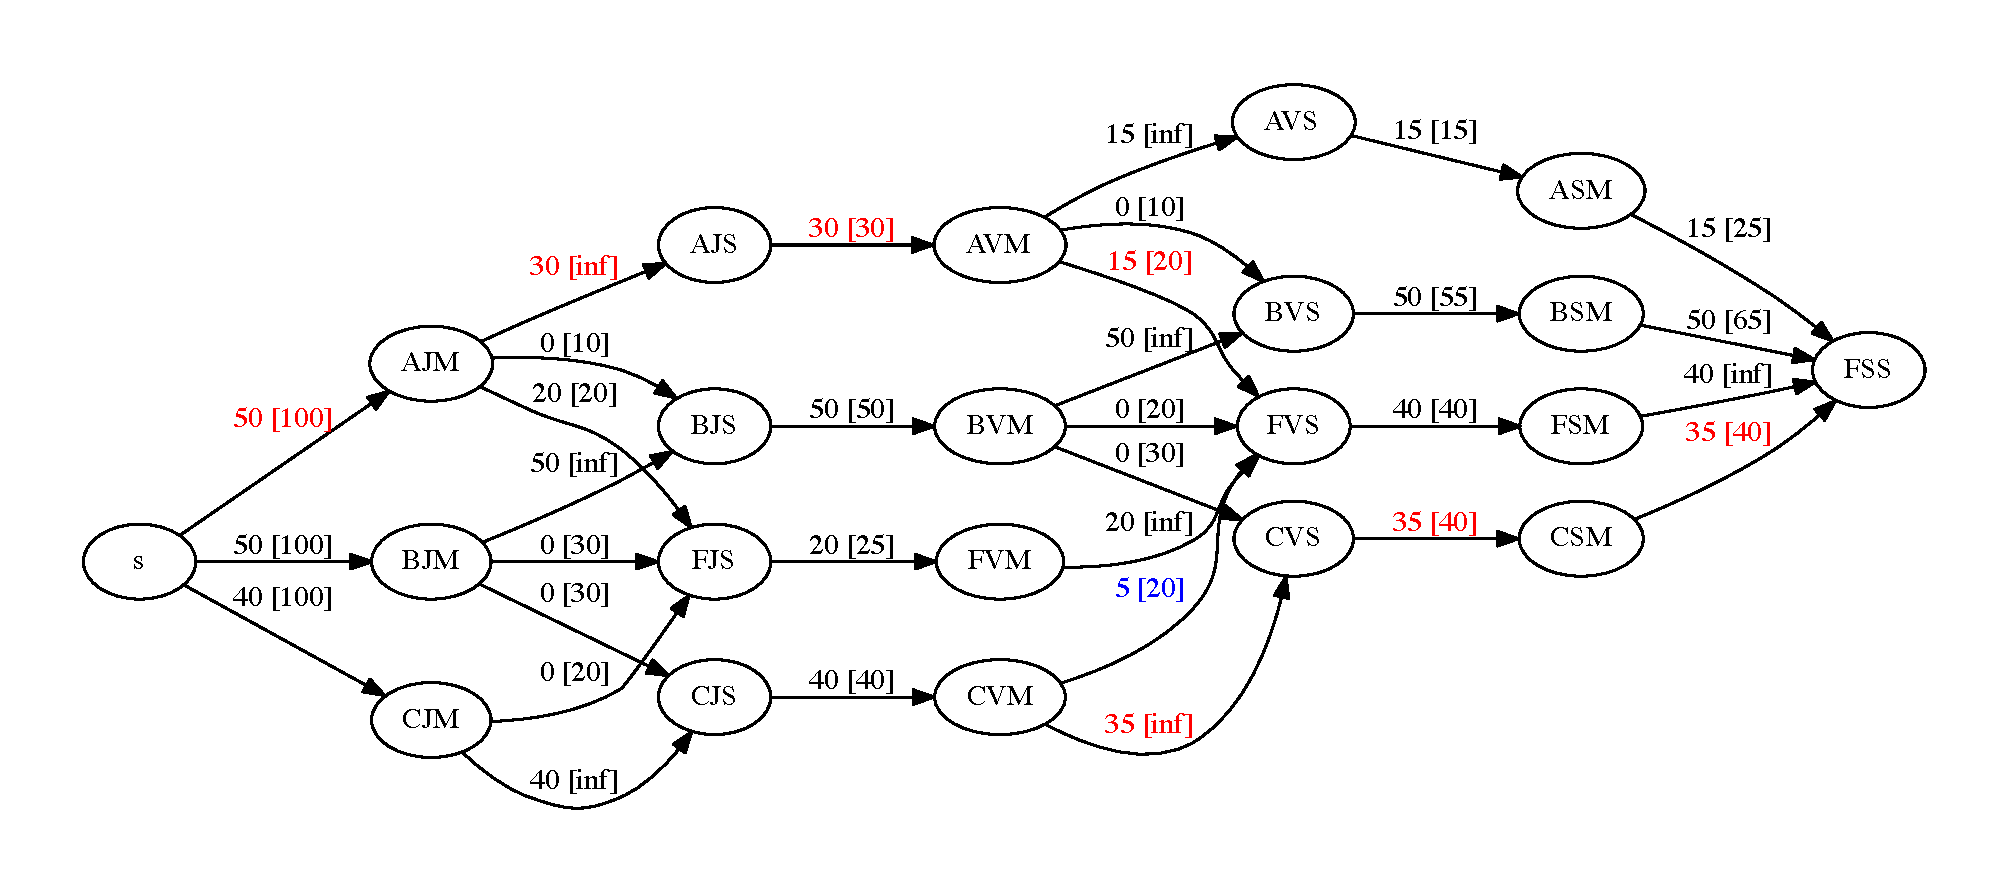
\includegraphics[width=\textwidth]{figs/pass-7.pdf}
	\caption{Sixième itération}
	\label{fig:pass:sept}
\end{center}
\end{figure}

\begin{figure}[h]
\begin{center}
	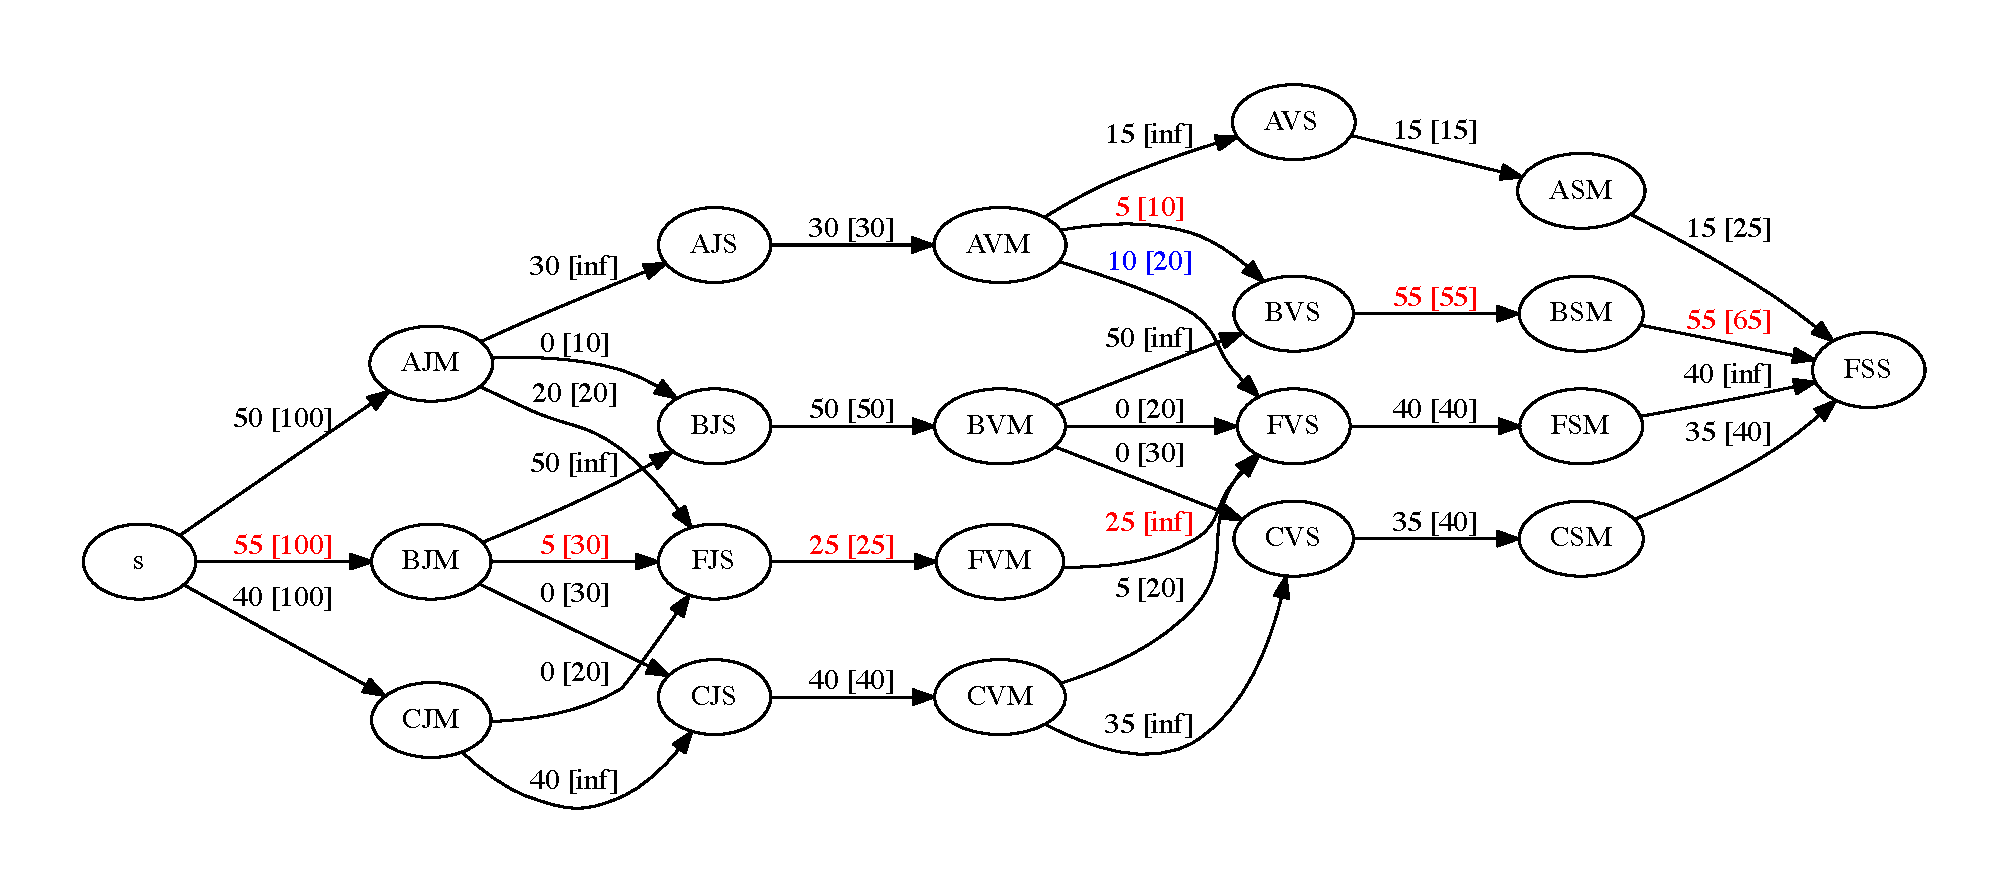
\includegraphics[width=\textwidth]{figs/pass-8.pdf}
	\caption{Septième itération}
	\label{fig:pass:huit}
\end{center}
\end{figure}

\begin{figure}[h]
\begin{center}
	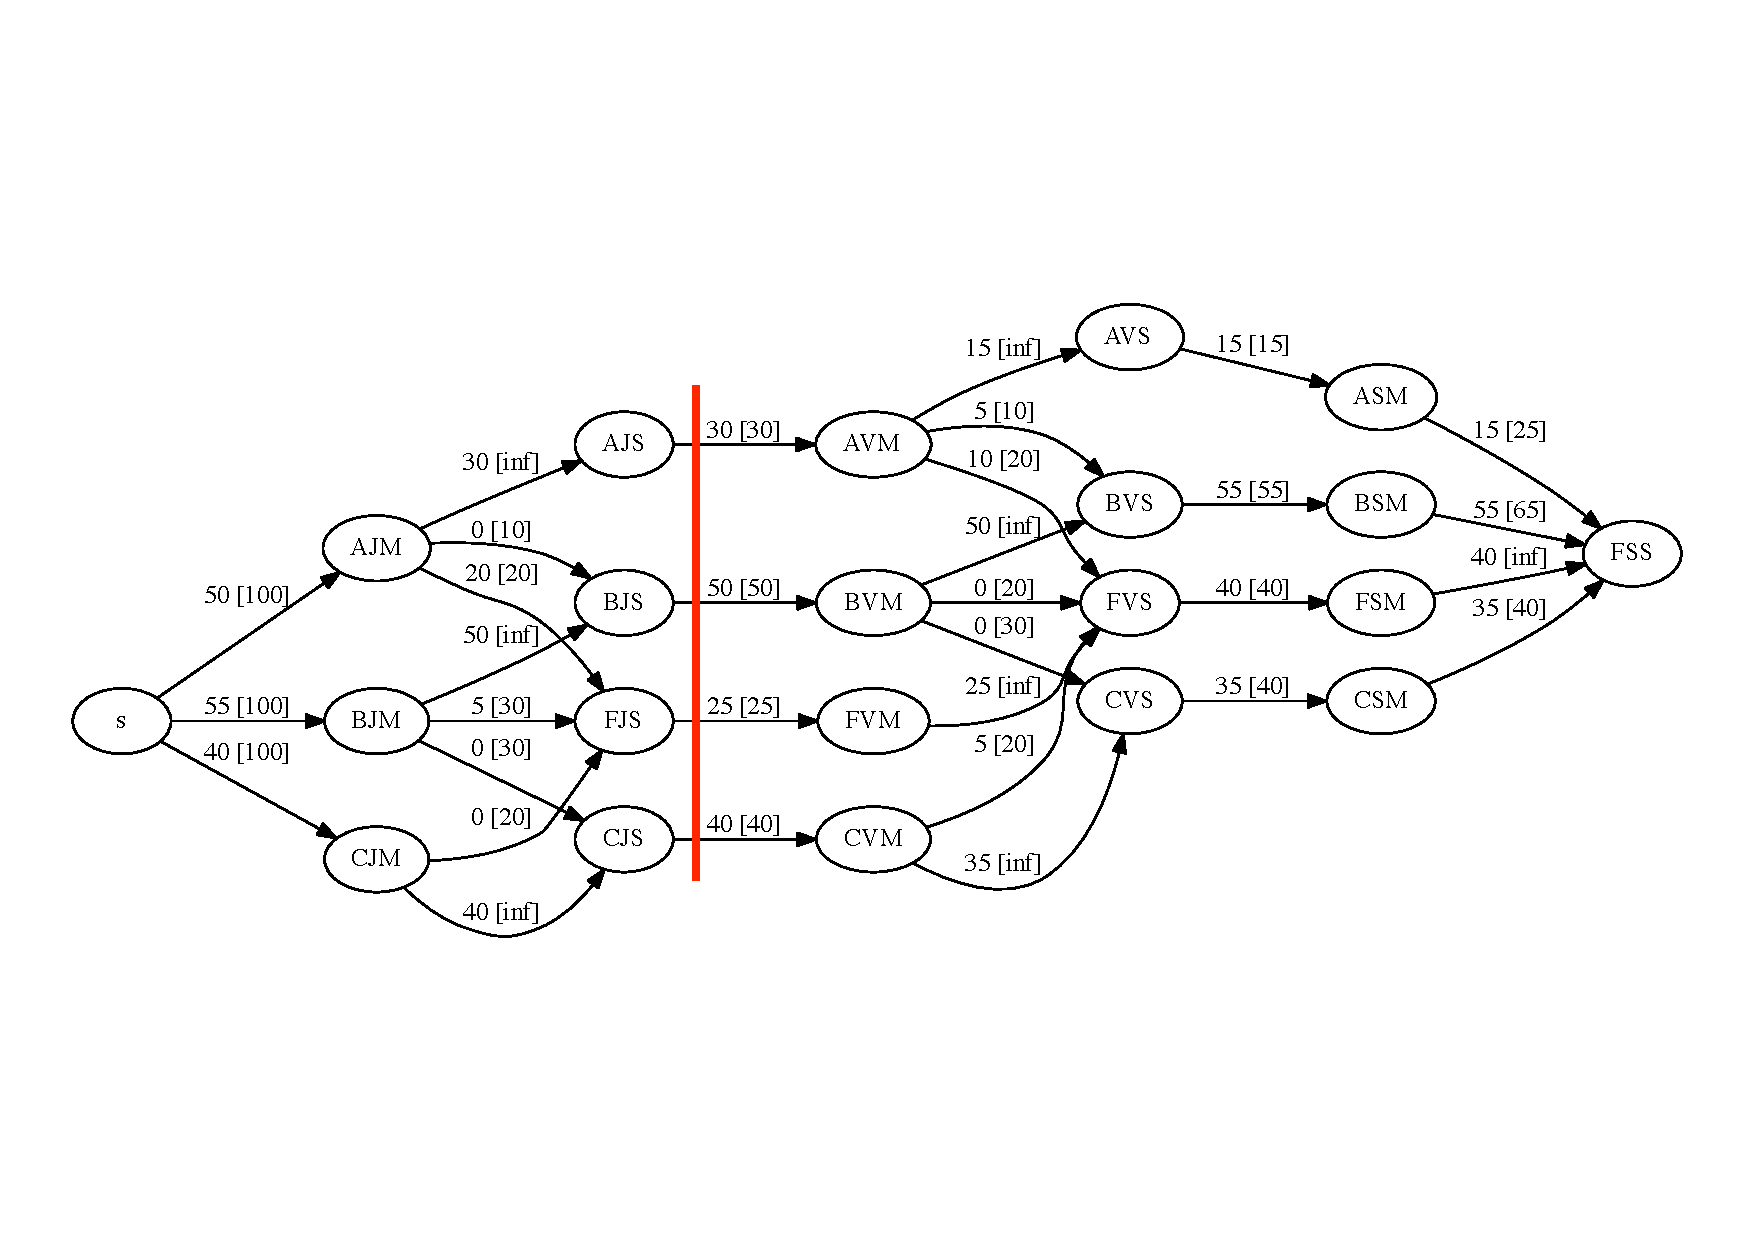
\includegraphics[width=\textwidth]{figs/pass-9.pdf}
	\caption{Flot final et coupe minimale}
	\label{fig:pass:neuf}
\end{center}
\end{figure}

\clearpage


\end{document}
%%% Local Variables: 
%%% mode: latex
%%% TeX-master: t
%%% End: 
